\documentclass[manuscript,screen,review]{acmart}
% \documentclass[manuscript,review,anonymous]{acmart}

%anonymous change
\AtBeginDocument{%
  \providecommand\BibTeX{{%
    \normalfont B\kern-0.5em{\scshape i\kern-0.25em b}\kern-0.8em\TeX}}}


\setcopyright{acmcopyright}
\copyrightyear{2023}
\acmYear{2023}
\acmDOI{XXXXXXX.XXXXXXX}

\acmConference[CHI '24]{Make sure to enter the correct
  conference title from your rights confirmation emai}{May 11--16,
  2024}{Honolulu, Hawaii}

\acmBooktitle{Hawaii' 24: ACM (Association of Computing Machinery) CHI conference on Human Factors in Computing Systems ,
 May 11--16,2024, Honolulu, Hawaii} 
\acmPrice{15.00}
\acmISBN{978-1-4503-XXXX-X/18/06}


\usepackage{multicol}
\usepackage{multirow}
\usepackage{array}
\usepackage{cleveref}
\usepackage{subcaption}
\usepackage{xcolor}
\usepackage{enumitem}
\usepackage{multirow}
\usepackage{subcaption}

%%
%% Submission ID.
%% Use this when submitting an article to a sponsored event. You'll
%% receive a unique submission ID from the organizers
%% of the event, and this ID should be used as the parameter to this command.
%%\acmSubmissionID{123-A56-BU3}

%%
%% For managing citations, it is recommended to use bibliography
%% files in BibTeX format.
%%
%% You can then either use BibTeX with the ACM-Reference-Format style,
%% or BibLaTeX with the acmnumeric or acmauthoryear sytles, that include
%% support for advanced citation of software artefact from the
%% biblatex-software package, also separately available on CTAN.
%%
%% Look at the sample-*-biblatex.tex files for templates showcasing
%% the biblatex styles.
%%

%%
%% The majority of ACM publications use numbered citations and
%% references.  The command \citestyle{authoryear} switches to the
%% "author year" style.
%%
%% If you are preparing content for an event
%% sponsored by ACM SIGGRAPH, you must use the "author year" style of
%% citations and references.
%% Uncommenting
%% the next command will enable that style.
%%\citestyle{acmauthoryear}

%%
%% end of the preamble, start of the body of the document source.
\begin{document}


\title{\textit{Is your AI really Creative?} Evaluating Creative Writing in the age of Large Language Models}


\author{Tuhin Chakrabarty}
\email{tuhin.chakr@cs.columbia.edu}
\affiliation{%
  \institution{Columbia University}
  \country{USA}
}

\author{Phillippe Laban}
\affiliation{%
  \institution{Salesforce AI Research}
  \country{USA}
}

\author{Divyansh Agarwal}
\affiliation{%
  \institution{Salesforce AI Research}
  \country{USA}
}

\author{Smaranda Muresan}
\email{smara@cs.columbia.edu}
\affiliation{%
  \institution{Columbia University}
  \country{USA}
}

\author{Chien-Sheng Wu}
\affiliation{%
  \institution{Salesforce AI Research}
  \country{USA}
}

% \renewcommand{\shortauthors}{Trovato and Tobin, et al.}


\begin{abstract}
Creativity is often associated with other markers of distinction, such as genius, imagination or originality.Eminent philosopher Vilém Flusser says "Only one who writes lines can think logically, calculate, criticize, pursue knowledge, philosophize.". Researchers have demonstrated that the current pile of large language models can  not only write academic essays, emails, cover letters but even poetry, fiction or screenplays. Unlike other forms of writing, creative writing places a much higher value on doing unexpected things that confound and delight the reader, typically contradicting the auto-regressive nature of LLMs. In spite of this there has been substantial discussion at the intersection of AI and creative writing, especially with researchers from Open-AI stating that creative writers and authors have extraordinarily high "exposure" to disruption from AI tools \cite{eloundou2023gpts}. Creativity is often difficult to evaluate because it is a complex, multifaceted concept that is deeply subjective, contextual, and hard to judge objectively. To tackle this, we interview 8 creative writing experts to elicit measures for evaluating creative writing. These measures are grounded in existing theoretical research on cognitive psychology for measuring creativity. We then recruit creative writing experts to utilize these measures to evaluate stories written by LLM's vs professional writers on the same plot. Our results show concerning trends that LLM generated stories are often of much poorer quality across several dimensions of creativity when compared to those written by professional writers. Additionally we also show that experts can easily identify stories written by AI vs those by professional writers. We also simulate the same evaluation using LLMs, demonstrating significant disagreement with creative writing experts thereby suggesting that LLMs are not aligned with expert humans across judgments about creativity.
\end{abstract}

%%
%% The code below is generated by the tool at http://dl.acm.org/ccs.cfm.
%% Please copy and paste the code instead of the example below.
%%

\begin{CCSXML}
<ccs2012>
   <concept>
       <concept_id>10003120.10003121.10011748</concept_id>
       <concept_desc>Human-centered computing~Empirical studies in HCI</concept_desc>
       <concept_significance>500</concept_significance>
       </concept>
   <concept>
       <concept_id>10003120.10003130.10011762</concept_id>
       <concept_desc>Human-centered computing~Empirical studies in collaborative and social computing</concept_desc>
       <concept_significance>500</concept_significance>
       </concept>
   <concept>
       <concept_id>10010147.10010178.10010179.10010182</concept_id>
       <concept_desc>Computing methodologies~Natural language generation</concept_desc>
       <concept_significance>300</concept_significance>
       </concept>
 </ccs2012>
\end{CCSXML}

\ccsdesc[500]{Human-centered computing~Empirical studies in HCI}
\ccsdesc[500]{Human-centered computing~Empirical studies in collaborative and social computing}
\ccsdesc[300]{Computing methodologies~Natural language generation}

% Author Keywords
\keywords{Human-AI collaboration, Large Language Models, Story Writing, Natural Language Generation, Evaluation, Creativity}% Print the classficiation codes

%% A "teaser" image appears between the author and affiliation
%% information and the body of the document, and typically spans the
%% page.
\begin{teaserfigure}
    \small
    \centering
  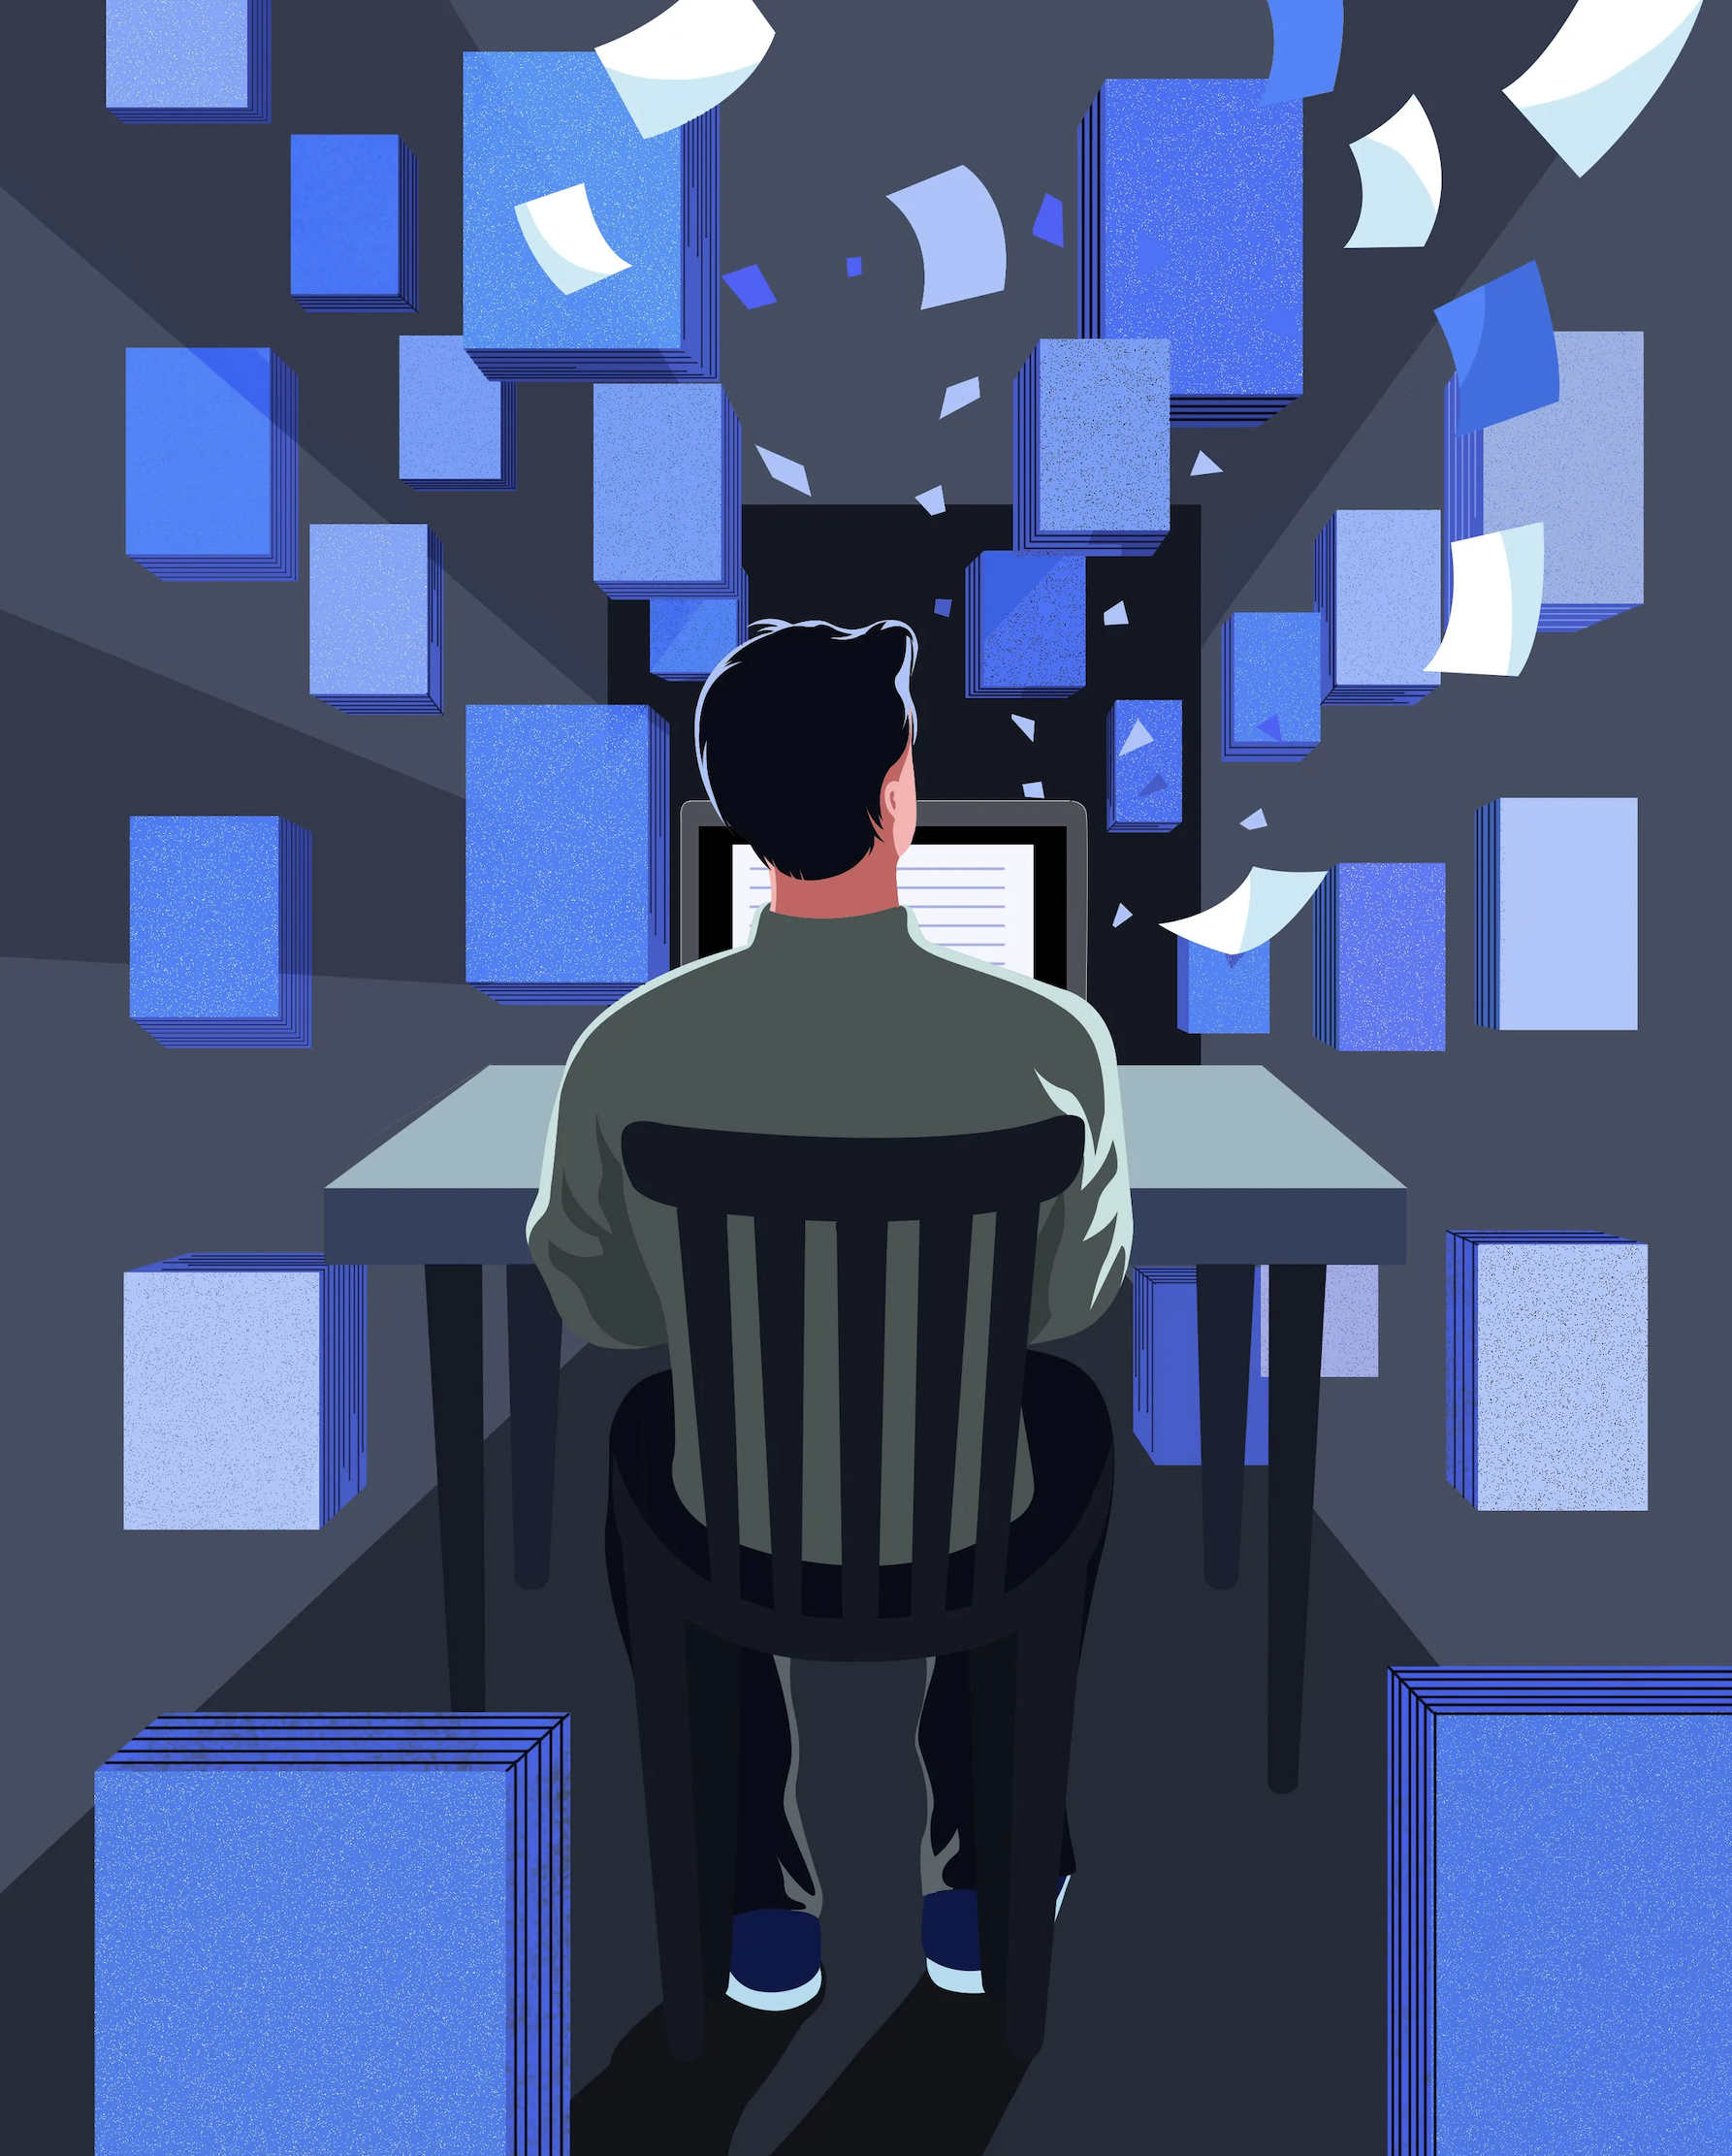
\includegraphics[width=0.35\textwidth]{sample-ai}
  \caption{\href{https://www.newyorker.com/culture/cultural-comment/the-computers-are-getting-better-at-writing}{The Computers Are Getting Better at Writing (The NewYorker)}}
  \Description{Enjoying the baseball game from the third-base
  seats. Ichiro Suzuki preparing to bat.}
  \label{fig:teaser}
\end{teaserfigure}

\received{20 February 2007}
\received[revised]{12 March 2009}
\received[accepted]{5 June 2009}


\maketitle

\newcommand{\ctask}{c_{\text{task}}}
\newcommand{\cmodel}{c_{\text{model}}}

\newcommand{\ms}{\mathscr}
\newcommand{\mc}{\mathcal}
\newcommand{\mf}{\mathfrak}

\newcommand{\bs}{\backslash}
\newcommand{\nsg}{\unlhd}
\newcommand{\ov}{\overline}

\newcommand{\N}{\mathbb{N}}
\newcommand{\R}{\mathbb{R}}
\newcommand{\Z}{\mathbb{Z}}
\newcommand{\Q}{\mathbb{Q}}
\newcommand{\F}{\mathbb{F}}
\newcommand{\C}{\mathbb{C}}

\newcommand{\Zp}{\Z^+}

\newcommand{\Rom}{\R^\omega}
\newcommand{\Rinf}{\R^\infty}

\newcommand{\linf}{\ell_\infty}
\newcommand{\lp}{\ell_p}
\newcommand{\lone}{\ell_1}

\newcommand{\dinf}{d_\infty}

\newcommand{\hess}{\nabla^2}
\newcommand{\diag}{\text{diag}}

\newcommand{\blone}{\textbf{1}}

\newcommand{\omn}{\omega_n}


\newcommand{\ip}{\langle\,,\rangle}

\newcommand{\mcP}{\mc{P}}
\newcommand{\mcS}{\mc{S}}
\newcommand{\mcB}{\mc{B}}
\newcommand{\mcC}{\mc{C}}
\newcommand{\mcF}{\mc{F}}
\newcommand{\mcI}{\mc{I}}
\newcommand{\mcE}{\mc{E}}
\newcommand{\mcA}{\mc{A}}
\newcommand{\mcL}{\mc{L}}


\newcommand{\aln}{{\aleph_0}}

\newcommand{\Rn}{\mathbb{R}^n}
\newcommand{\Rnn}{\R^{n \times n}}
\newcommand{\eps}{\epsilon}
\newcommand{\norm}[1]{||#1||}
\newcommand{\pnorm}[1]{\norm{#1}_p}
\newcommand{\qnorm}[1]{\norm{#1}_q}
\newcommand{\onorm}[1]{\norm{#1}_1}
\newcommand{\inorm}[1]{||#1||_\infty}
\newcommand{\tnorm}[1]{\norm{#1}_2}
\newcommand{\shyone}[1]{\frac{#1}{#1}}
\newcommand{\shyzero}[1]{#1 - #1}
\newcommand{\floor}[1]{\left\lfloor #1 \right\rfloor}
\newcommand{\ceil}[1]{\left\lceil #1 \right\rceil}
\newcommand{\pd}[1]{\frac{\partial}{\partial #1}}
\newcommand{\pdn}[2]{\frac{\partial^{#2}}{\partial {#1}^{#2}}}
\newcommand{\pdm}[2]{\frac{\partial^{#2}}{\partial {#1}}}
\newcommand{\diex}{\pd{x}}
\newcommand{\diey}{\pd{y}}
\newcommand{\diez}{\pd{z}}
\newcommand{\ddx}{\frac{d}{dx}}
\newcommand{\mat}[1]{\begin{bmatrix} #1 \end{bmatrix}}
\newcommand{\EX}{\mathbb{E}}
\newcommand{\Var}[1]{\text{Var}(#1)}
\newcommand{\recip}[1]{\frac{1}{#1}}
\newcommand{\inv}[1]{#1^{-1}}
\newcommand{\finv}{\inv{f}}
\newcommand{\set}[1]{\{#1\}}
\newcommand{\braces}[1]{\left\{ #1 \right\}}
\newcommand{\setstar}[1]{\{#1\}^*}
\newcommand{\jjlim}[2]{\lim_{#2 \rightarrow #1}}
\newcommand{\jjpar}[1]{\left( #1 \right)}
\newcommand{\jjbra}[1]{\left\{ #1 \right\}}
\newcommand{\jjabs}[1]{\left\lvert #1 \right\rvert}
\newcommand{\jjcases}[1]{\begin{cases} #1 \end{cases}}
\newcommand{\jjalg}[2]{ 
    
    \noindent {#1}
        \begin{algorithmic}[1]
            #2
        \end{algorithmic}
}
\newcommand{\jjbold}[1]{{\bf #1}}


\newcommand{\LT}[1]{\mathcal{L}\set{#1}}
\newcommand{\LTi}[1]{\mathcal{L}^{-1}\set{#1}}

\newcommand{\ket}[1]{\left\lvert #1 \right\rangle}
\newcommand{\kphi}{\ket{\phi}}
\newcommand{\kpsi}{\ket{\psi}}
\newcommand{\kOmega}{\ket{\Omega}}
\newcommand{\kone}{\ket{1}}
\newcommand{\koone}{\ket{11}}
\newcommand{\kzero}{\ket{0}}
\newcommand{\kzzero}{\ket{00}}
\newcommand{\kzone}{\ket{01}}
\newcommand{\kozero}{\ket{10}}

\newcommand{\bra}[1]{\left\langle #1 \right\rvert}
\newcommand{\bphi}{\bra{\phi}}
\newcommand{\bpsi}{\bra{\psi}}
\newcommand{\bOmega}{\bra{\Omega}}
\newcommand{\bone}{\bra{1}}
\newcommand{\boone}{\bra{11}}
\newcommand{\bzero}{\bra{0}}
\newcommand{\bzzero}{\bra{00}}
\newcommand{\bzone}{\bra{01}}
\newcommand{\bozero}{\bra{10}}


\newcommand{\matX}{\mat{0 & 1 \\ 1 & 0}}
\newcommand{\matY}{\mat{0 & -i \\ i & 0}}
\newcommand{\matZ}{\mat{1 & 0 \\ 0 & -1}}
\newcommand{\matH}{\irtwo\mat{1 & 1 \\ 1 & -1}}
\newcommand{\matI}{\mat{1 & 0 \\ 0 & 1}}
\newcommand{\matCNOT}{\mat{1 & 0 & 0 & 0 \\ 0 & 1 & 0 & 0 \\ 0 & 0 & 0 & 1 \\ 0 & 0 & 1 & 0}}
\newcommand{\matUCNOT}{\mat{1 & 0 & 0 & 0 \\ 0 & 0 & 0 & 1 \\ 0 & 0 & 1 & 0 \\ 0 & 1 & 0 & 0}}


\newcommand{\rt}{\sqrt{2}}
\newcommand{\half}{\frac{1}{2}}
\newcommand{\third}{\frac{1}{3}}
\newcommand{\tthird}{\frac{2}{3}}
\newcommand{\fourth}{\frac{1}{4}}
\newcommand{\fifth}{\frac{1}{5}}
\newcommand{\sixth}{\frac{1}{6}}
\newcommand{\seventh}{\frac{1}{7}}
\newcommand{\eighth}{\frac{1}{8}}


\newcommand{\irtwo}{\frac{1}{\sqrt{2}}}
\newcommand{\irtwoa}[1]{\frac{#1}{\sqrt{2}}}
\newcommand{\itrtwo}{\frac{1}{2\sqrt{2}}}


\newcommand{\jjdag}[1]{#1^\dagger}

\newcommand{\softmax}[1]{\text{softmax}\jjpar{#1}}
\newcommand{\SDP}[1]{\text{SDP}\jjpar{#1}}
\newcommand{\LSE}[1]{\text{LSE}\jjpar{#1}}

\newcommand{\seqlen}{\text{seqlen}}
\section{Introduction}
\label{sec:intro}


Transformers, in particular decoder-only models (e.g.\ GPT~\citep{brown2020language}, Llama~\citep{touvron2023llama}) which process input sequences in a causal fashion, are one of the main drivers of modern deep learning's success.
Numerous approaches attempt to approximate the core attention layer to address its efficiency issues~\citep{tay2022efficient}, such as scaling quadratically in sequence length during training and requiring a cache of size linear in sequence length during autoregressive generation.
In parallel, a class of alternative sequence models, structured state-space models (SSMs), have emerged with linear scaling in sequence length during training and constant state size during generation.
They show strong performance on long-range tasks (e.g. S4~\citep{gu2022efficiently}) and recently matched or beat Transformers on language modeling (e.g. Mamba \citep{gu2023mamba}) at small to moderate scale.
However, the development of SSMs have appeared disjoint from the community's collective effort to improve Transformers, such as understanding them theoretically as well as optimizing them on modern hardware.
As a result, it is more difficult to understand and experiment with SSMs compared to Transformers, and it remains challenging to train SSMs as efficiently as Transformers from both an algorithmic and systems perspective.


Our main goal is to develop a rich body of theoretical connections between structured SSMs and variants of attention.
This will allow us to transfer algorithmic and systems optimizations originally developed for Transformers to SSMs, towards the goal of building foundation models that perform better than Transformers while scaling more efficiently in sequence length.
A milestone contribution in this direction was the \textbf{Linear Attention (LA)} framework \citep{katharopoulos2020transformers},
which derived a connection between autoregressive attention and linear RNNs
by showing the equivalence between ``dual forms'' of quadratic kernelized attention and a particular linear recurrence.
This duality allows new capabilities such as the ability to have both efficient parallelizable training and efficient autoregressive inference.
In the same spirit, this paper provides multiple viewpoints connecting linear-complexity SSMs with quadratic-complexity forms to combine the strengths of SSMs and attention.%
\footnote{Technically speaking, these connections only relate to certain flavors of attention; the title of this paper is an homage to \citet{katharopoulos2020transformers} which first showed that ``Transformers are RNNs''.}

\iftoggle{arxiv}{
\begin{wrapfigure}{R}{0.48\linewidth}
  \begin{center}
    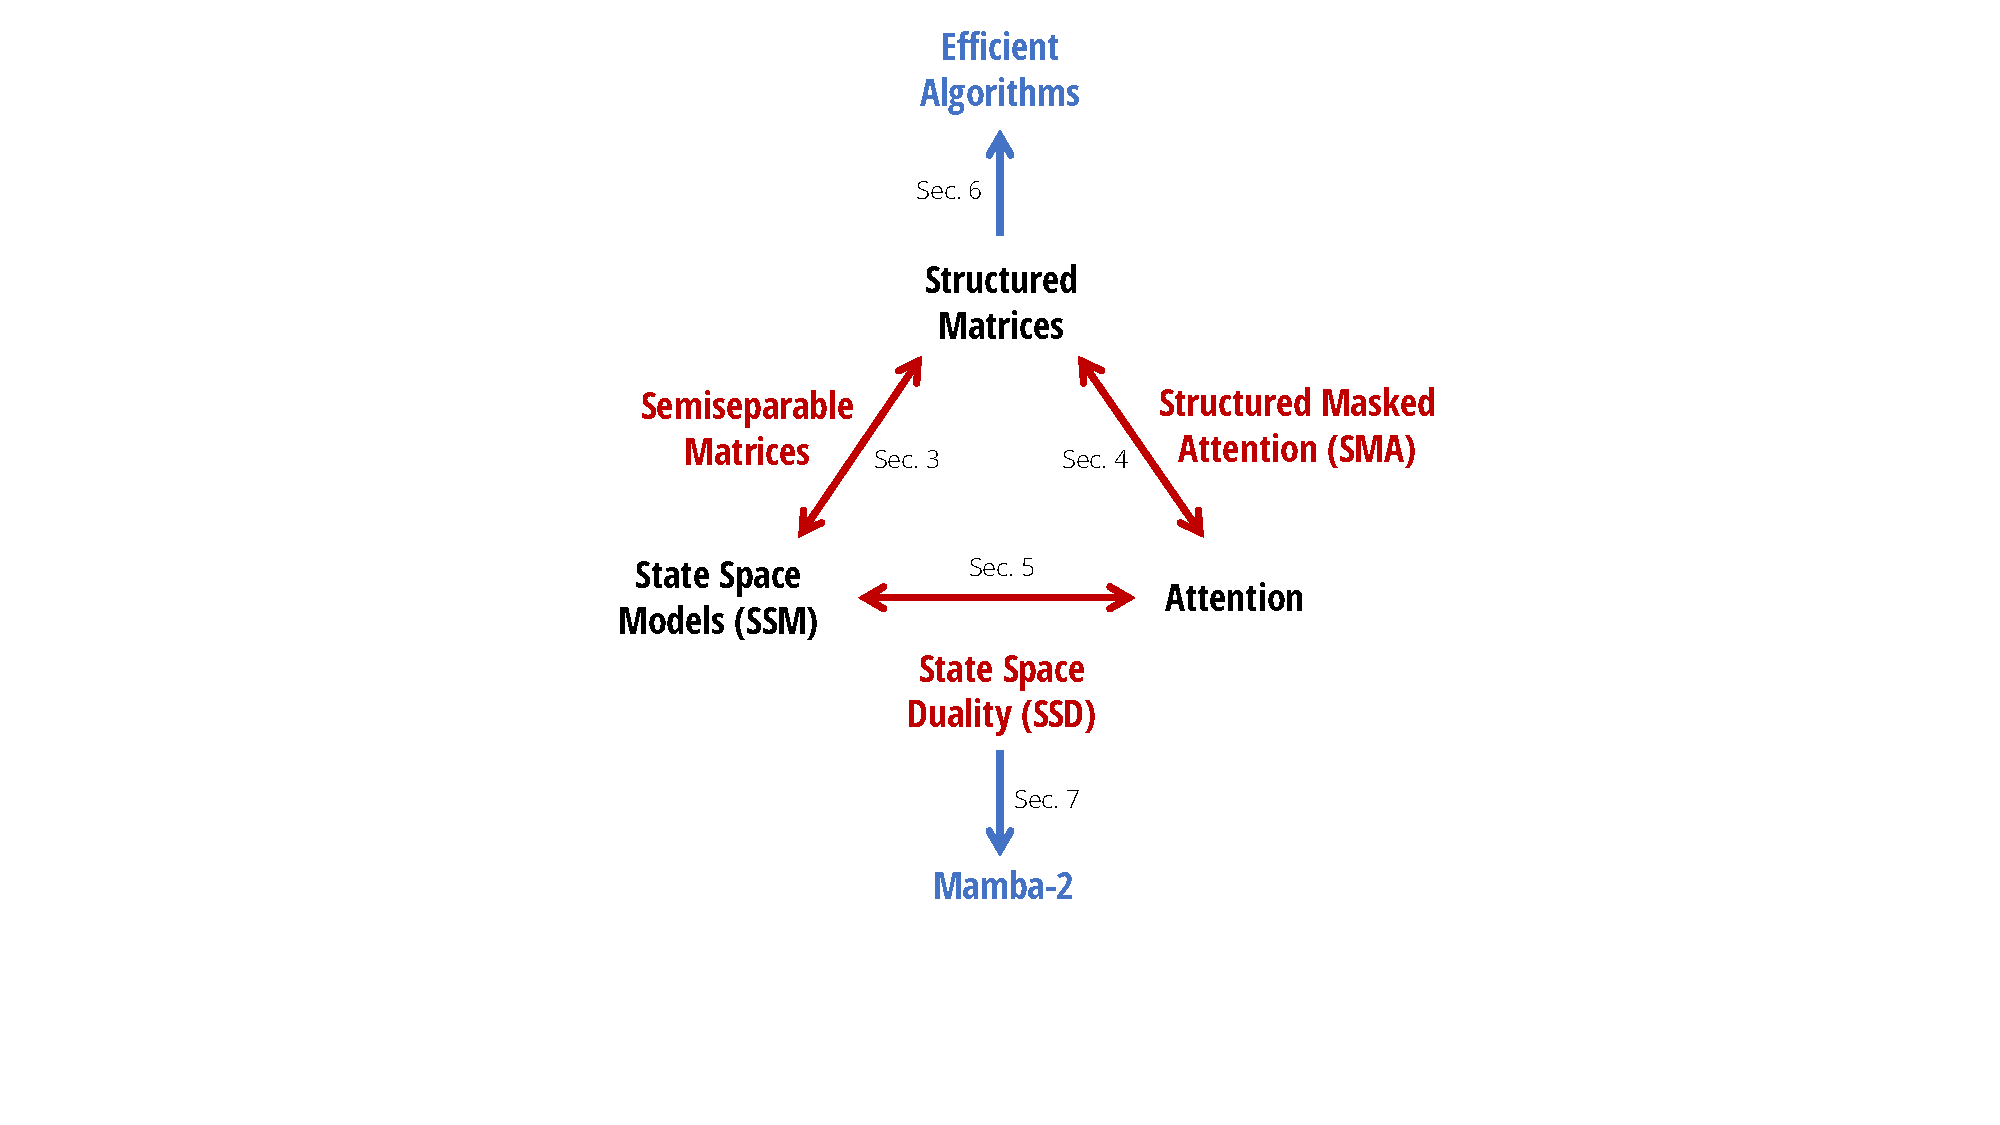
\includegraphics[width=\linewidth]{fig/ssd_roadmap.pdf}
  \end{center}
  \caption{
    (\textbf{Structured State-Space Duality}.)
    This paper fleshes out the relationship between state space models and attention through the bridge of structured matrices.
  }
  \label{fig:roadmap}
\end{wrapfigure}
}{}

\para{State Space Duality.}
Our framework connecting structured SSMs and variants of attention, which we call \textbf{structured state space duality} (SSD),
is made through the abstractions of \textbf{structured matrices}:
matrices with subquadratic parameters and multiplication complexity.
We develop two broad frameworks for representing sequence models, one as matrix transformations and one as tensor contractions, which each reveal different perspectives of the duality.
Our technical contributions include:
\begin{itemize}[leftmargin=*,itemsep=0pt,topsep=0pt]
  \item We show an equivalence between state space models and a well-studied family of structured matrices called \textbf{semiseparable matrices}\iftoggle{arxiv}{ (\cref{sec:ssm})}{}.
    This connection is at the heart our framework, revealing new properties and algorithms for SSMs. A central message of this paper is that \emph{different methods of computing state space models can be reframed as various matrix multiplication algorithms on structured matrices}.
  \item We significantly improve the theory of linear attention~\citep{katharopoulos2020transformers}.
    We first provide an incisive proof of its recurrent form through the language of tensor contractions, and then generalize it to a new family of \textbf{structured masked attention (SMA)}\iftoggle{arxiv}{ (\cref{sec:attention})}{}.
  \item We connect SSMs and SMA, showing that they have a large intersection that are duals of each other, possessing both SSM-like linear and attention-like quadratic forms\iftoggle{arxiv}{ (\cref{sec:ssd})}{}.
    \iftoggle{arxiv}{We also prove that any kernel attention method possessing a fast recurrent form must be an SSM.}{}
\end{itemize}


Beyond its intrinsic theoretical value, our framework opens up a broad set of directions for understanding and improving sequence models.

\para{Efficient Algorithms.}
First and most importantly, our framework exposes new efficient and easily-implementable algorithms for computing SSMs\iftoggle{arxiv}{ (\cref{sec:efficient})}{}.
We introduce a new \textbf{SSD algorithm}, based on block decompositions of semiseparable matrices, that takes advantage of both the linear SSM recurrence and quadratic dual form, obtaining optimal tradeoffs on all main efficiency axes (e.g. training and inference compute, memory usage, and ability to leverage matrix multiplication units on modern hardware).
A dedicated implementation of SSD is $2-8\times$ faster than the optimized selective scan implementation of Mamba, while simultaneously allowing for much larger recurrent state sizes ($8\times$ the size of Mamba or even higher, with minimal slowdown).
SSD is highly competitive with optimized implementations of softmax attention (FlashAttention-2~\citep{dao2023flashattention2}), crossing over at sequence length 2K and 6$\times$ faster at sequence length 16K.


\iftoggle{arxiv}{
\para{Architecture Design.}
One major obstacle to adopting new architectures such as SSMs is the ecosystem tailored to Transformers, such as hardware-efficient optimization and parallelism techniques for large-scale training.
Our framework allows using established conventions and techniques for attention to build a vocabulary of architecture design choices for SSMs, and further improve them (\cref{sec:architecture}).
For example, we introduce the analog of heads from multi-head attention (MHA) to SSMs.
We show that the Mamba architecture is a \textbf{multi-input SSM (MIS)} that turns out to be analogous to \textbf{multi-value attention (MVA)}, and compare other variants of Mamba with different head structures.

We also use these ideas to make slight modifications to the Mamba block, which allows tensor parallelism to be implemented (e.g. in the style of Megatron~\citep{shoeybi2019megatron}).
The main ideas include introducing grouped-value attention (GVA) head structure, and moving all data-dependent projections to occur in parallel at the beginning of the block.


}{
  \para{Mamba-2.}
  Additionally, inspired by the connection between SSMs and Transformers, we slightly modify the neural network architecture of Mamba by moving all data-dependent projections to occur in parallel at the beginning of the block. %
}
The combination of the modified parallel Mamba block, together with using SSD as the inner SSM layer, results in the \textbf{Mamba-2} architecture.
We investigate Chinchilla scaling laws for Mamba-2 in the same setting as Mamba, finding that it Pareto dominates Mamba and Transformer++ in both perplexity and wall-clock time.
We additionally train a family of Mamba-2 models at varying sizes on the Pile, showing that it matches or outperforms Mamba and open source Transformers on standard downstream evaluations.
For example, Mamba-2 with 2.7B parameters trained on 300B tokens on the Pile outperforms Mamba-2.8B, Pythia-2.8B and even Pythia-6.9B trained on the same dataset.

\iftoggle{arxiv}{
\paragraph{Systems Optimizations.}
The SSD framework connects SSMs and Transformers, allowing us to leverage a rich body of work on systems optimizations developed for Transformers~(\cref{sec:systems}).
\begin{itemize}[leftmargin=*,itemsep=0pt,topsep=0pt]
  \item For example, Tensor Parallelism (TP) is an important model parallelism technique to train large Transformer models by splitting each layer across GPUs on the same node.
    We design Mamba-2 to be TP-friendly, reducing the number of synchronization point per block by half.
  \item For very long sequences whose activations do not fit on one device, sequence parallelism has been developed for the attention blocks.
    We describe how to train SSMs in general and Mamba-2 in particular with sequence parallelism, by passing the recurrent states between devices.
  \item For finetuning with examples of different lengths, for best efficiency, Transformer requires sophisticated techniques to remove padding tokens and perform attention on variable length sequences.
    We show how Mamba-2 can be trained with variable sequence lengths efficiently, requiring no padding tokens.
\end{itemize}
}{}

\cref{sec:experiments} empirically validates Mamba-2 on language modeling, training efficiency, and a difficult multi-query associative recall task~\citep{arora2024simple}.
Finally, in \cref{sec:related}, we provide an extended related work and discuss potential research directions opened up by our framework.

Model code and pre-trained checkpoints are open-sourced at \url{https://github.com/state-spaces/mamba}.






\section{Related work}

There is a rich prior literature on 
probabilistic programming languages (PPLs),
which extend probabilistic graphical models to
support more complex joint distributions whose size and ``shape''
can itself be stochastic (e.g., a graph
unrolled for a random number of iterations,
until a data-dependent stopping criterion is met).
PPLs extend traditional programming languages with the ability to {\it sample} from distributions and {\it observe} values of variables based on data (i.e. condition the model).
The semantics of sample and observe vary depending on the inference algorithm.
For more details, see  \citet{intro_ppl}.

Recently there has been an explosion of interest in large language models, such as 
GPT-3 \citep{gpt3} and PaLM \citep{palm}.
%\citep{lamda}.
These can be used for tasks such as ``zero-shot"
question-answering. In this setting, we 
provide the question $Q$ as a prompt to the LM,
and then sample answers from the model, 
which we denote by $p(A|Q,\theta)$,
where $\theta$ are the pre-trained model parameters.
Alternatively, we can compute the MAP answer,
$\hat{A} = \argmax_A p(A|Q,\theta)$.


To ensure the model ``does the right thing'',
we can provide a small training set of question-answer pairs,
$D = \{ (Q^m,A^m): m=1:M\}$ pairs.
This can be provided as extra context to the model,
provided in the text prompt, followed by sampling
from $p(A|Q,D,\theta)$.
We refer to this as ``few-shot prompting''.
We can also fine-tune the model parameters on $D$ to
get $\theta'$, and then sample
from $p(A|Q,\theta')$.

%We can improve performance on question answering tasks by encouraging the model
%chaining multiple LMs together,  % david: They don't actually do multiple calls, just prompt it to produce the aux variable directly.
%as illustrated in the
%Scratchpad \citep{scratchpads} and Chain of Thought \citep{chainofthought}  papers.
%These papers introduce an  an additional auxiliary ``thought''
%variable $T$ and then extend the model to have the form
%$P(A,T|Q) = P(A|T,Q)P(T|Q)$, where each conditional is computed
%using an LM.

We can improve performance by introducing an additional auxiliary ``thought'' variable,
and then extend the model to have the form $p(A,T|Q) = p(A|T,Q)p(T|Q)$, where each conditional is computed using an LM which includes its conditioning variables as a part of its input.
Work on scratchpads \citep{scratchpads} and chain of thought \citep{chainofthought} illustrate this, and finetune or prompt the LM to produce this auxiliary thought before answering.
%We can improve performance on question answering tasks by encouraging the model
%chaining multiple LMs together,  % david: They don't actually do multiple calls, just prompt it to produce the aux variable directly.
% These papers 
% variable $T$ 

We typically condition this on a small set
$D_S$ of  $(A^m,T^m,Q^m)$ triples,
and optionally a larger set $D_L$ of $(A^m, Q^m)$ pairs.
We then compute a distribution over answers to a test question
using
\begin{align}
\hat{p}(A|Q) = \sum_T 
\hat{p}(A|Q, T) \hat{p}(T|Q)
\label{eqn:probQA}
\end{align}
where $\hat{p}(\cdot) = p(\cdot|D_L,D_S,\theta)$
is the prior predictive distribution. (Scratchpad creates its prior predictive by fine-tuning, while Chain of Thought adds $D_S$ to the LM prompt.)

In practice, we cannot sum over all possible strings $T$
in \cref{eqn:probQA}.
The most common approach is to compute the MAP estimate
$\hat{T} = \argmax \hat{p}(T)$ using beam search,
and then to approximate the sum over $T$ with this single
value.
More recently, Self Consistency \citep{selfconsistency} 
proposed to sample multiple values for $T$
using forward sampling of $(A,T)$ given $Q$,
and then taking the answer $A$ that is most common
in this set\footnote{This bucketing is practical because most standard benchmarks have answers that are just a couple words.}.

PromptChainer \citep{promptchainer} proposes a visual interface for composing language models together, specifying control flow and prompting strategies for each node in a chain. Nodes may query language models or external systems. 
Socratic models \citep{socraticmodels} extends model chaining to the multimodal setting and demonstrates zero-shot abilities on tasks for which no single model exists.

The Eliciting Latent Knowledge proposal \citep{ELK} suggests making latent variables explicit, modelled using a Bayesian network, to improve interpretability and safety for advanced AI systems.
% Factored cognition \citet{factored_cognition}

\citet{ortega2021shaking} explains a formalism for LM finetuning with causal graphical models in order to extend the predictive capabilities of AI agents towards more adaptive behaviour. They focus on analysing an auto-regressive action (random variable) prediction scheme in the interactive setting of RL where a model is simultaneously a generator and predictor of data.

% \citet{language_feedback} incorporates language feedback to finetune models, and finds that learning is significantly more sample efficient. \ddohan{We view this feedback as an auxiliary variable which can be conditioned to inform inference.}

%\kevin{Omit RL refs since not relevant?}
%Incorporating human feedback into generative models remains an open problem. Reinforcement from human feedback has become a popular approach to finetuning models against human preferences. \citep{learning_to_summarize, anthropic_human_feedback} learn a surrogate model of human preferences and use PPO \citep{ppo} to finetune a language model to maximize this surrogate. Rather than using scalar feedback, \citet{language_feedback} incorporates language feedback to finetune models, and finds that learning is significantly more sample efficient. \ddohan{We view this feedback as an auxiliary variable which can be conditioned to inform inference.}
%\todo{ddohan: consider adding back in language feedback ref}

%\citep{Levine2022} presents some very recent work on using frozen LMs in various ways.\rif{Suggest we cut this if we don't have more to say.}






\section{Designing Tests for Creative Writing} \label{sec:approach}
\subsection{Rethinking Torrance Test of Creative Thinking}
Built on J.P. Guilford's work and created by Ellis Paul Torrance, the Torrance Tests of Creative Thinking, a test of creativity, originally involved simple tests of divergent thinking and other problem-solving skills, which were scored on four scales:

\begin{figure*}
\centering
\small
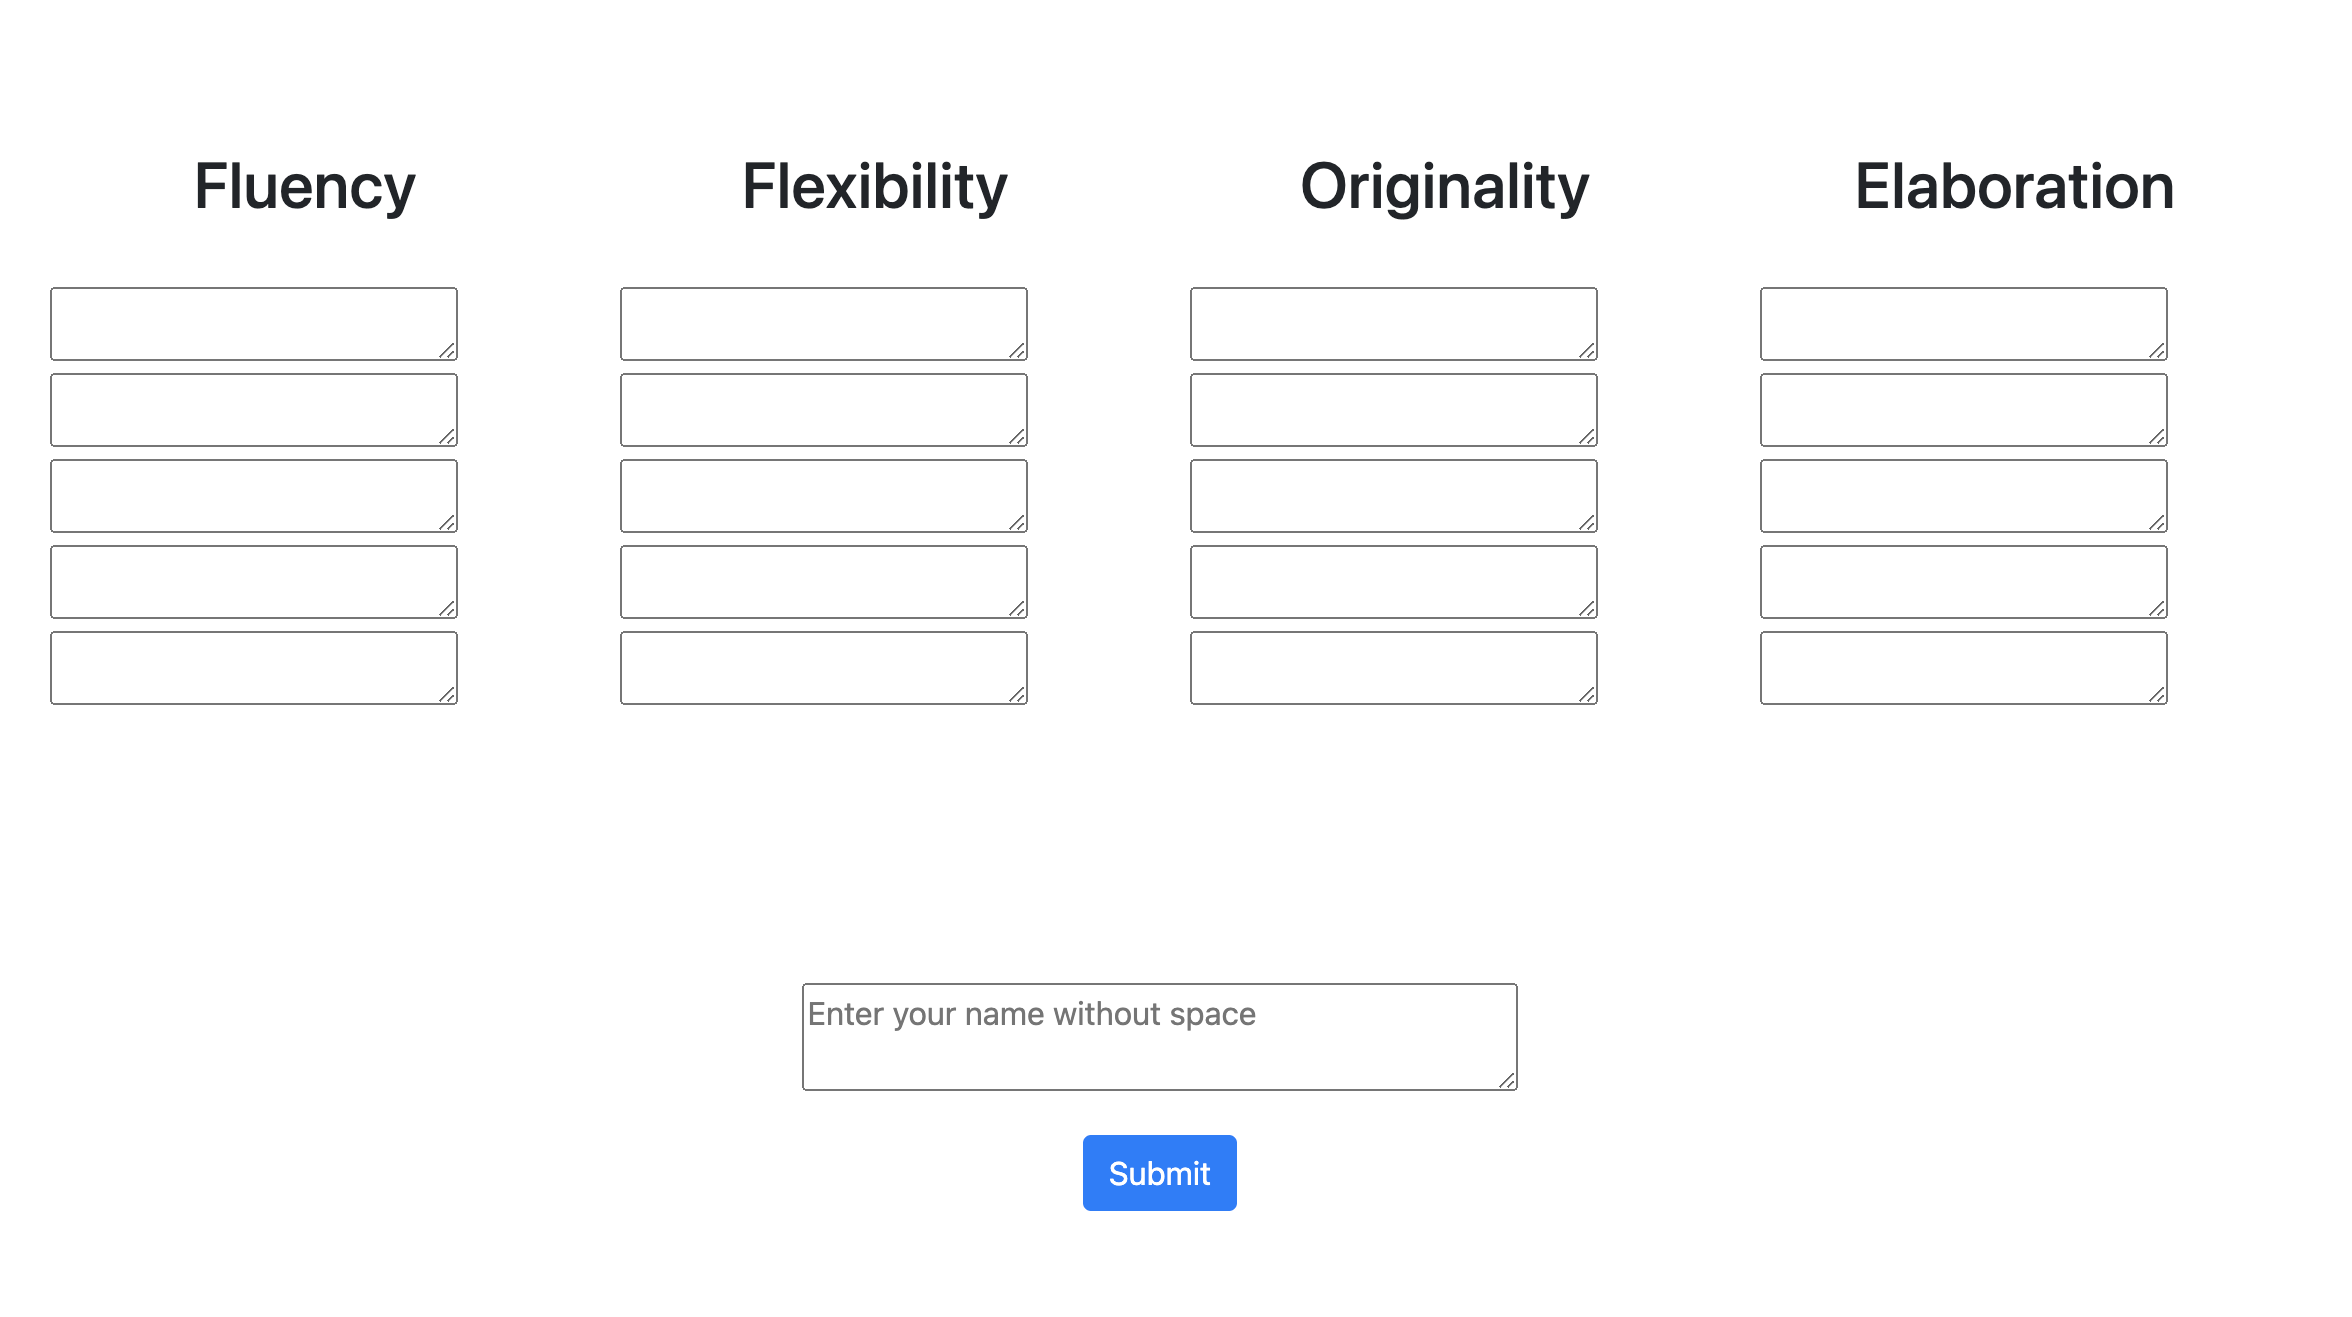
\includegraphics[width=0.8\textwidth]{figures/interface.png}
\caption{\label{fig:interface}Interface to collect Creativity measurements across the four-dimensional analytical framework derived from the Torrance Test of Creative Thinking}
\end{figure*}

\begin{itemize}
    \item Fluency. The total number of interpretable, meaningful, and relevant ideas generated in response to the stimulus.
    \item  Flexibility. The number of different categories of relevant responses.
    \item Originality. The statistical rarity of the responses.
    \item Elaboration. The amount of detail in the responses.
\end{itemize}

While prior work \cite{10.1145/3313831.3376495,10.1145/1978942.1979048,Beketayev2016ScoringDT} has utilized Torrance Test of Creative Thinking in other domains, it hasn't been used to evaluate creative writing. Even though the overall dimensions are generalizable across various forms of art, there are measures specific to creative writing along these dimensions that require the existing definitions to be revised and expanded. For this we recruit experts in creative writing. 

\subsection{Participant Recruitment}
In prior work \cite{gero2023social} has argued that the definition of an ‘expert’ or ‘amateur’ creative writer is difficult in a field that has unclear professional delineations.Though it could be feasible to enlist individuals self-identifying as creative professionals, our requirements necessitated the procurement of participants possessing an intricate and analytical comprehension of the creative writing process. Accordingly, we delimited our participant acquisition to those possessing either a structured educational background in creative writing (for instance, a Master of Fine Arts in Creative Writing), traditionally published authors \footnote{We do not recruit self-published authors}, or lecturers/professors instructing Fiction Writing at the university level.Our recruitment thus resulted in participants who have published novels with leading publishing giants, students enrolled in top MFA programs in the United States, University professors teaching Fiction Writing and screenwriters from prime-time network. Participants were recruited through \textit{User Interviews} (a professional freelancing website) and were paid 70\$ for a taking part in an hour long survey. Table \ref{surveyprof} shows our recruited participants.

\begin{table}[!ht]
\centering
\small
\def\arraystretch{1.35}
\parbox{.45\linewidth}{\begin{tabular}{ll}
\hline
ID & Profession                  \\ \hline
W1 & Professor of Creative Writing \\ \hline
W2 & Professor of Creative Writing \\ \hline
W3 & Lecturer in Creative Writing  \\ \hline
W4 & MFA Fiction Student           \\ \hline
W5 & MFA Fiction Student           \\ \hline
W6 & MFA Fiction Student           \\ \hline
W7 & Author                        \\ \hline
W8 & ScreenWriter                  \\ \hline
\end{tabular}
\vspace{2ex}
\caption{\label{surveyprof}Background of Participants recruited for collecting judgements about Creativity across the dimensions of Torrance Test}
}
\quad\quad\quad\quad
\parbox{.45\linewidth}
{\begin{tabular}{ll}
\hline
Cluster & Participants                  \\ \hline
Narrative Pacing & W4,W6,W7 \\ \hline
\begin{tabular}[c]{@{}l@{}}Understandability\\ \& Coherence\end{tabular}  & W3,W7 \\ \hline
\begin{tabular}[c]{@{}l@{}}Language Proficiency\\ \& Literary Devices\end{tabular}  & W4,W2  \\ \hline
Narrative Ending & W3           \\ \hline
Scene vs Summary & W2,W5,W8          \\ \hline\hline
Structural Flexibility & W3,W7,W8           \\ \hline
Perspective \& Voice Flexibility & W3,W6                        \\ \hline
Emotional Flexibility & W3                  \\ \hline\hline
Originality in Theme/Content & W3                  \\ \hline
Originality in Thought & W1,W2,W3,W5,W7                  \\ \hline
Originality in Form/Structure & W2,W4                  \\ \hline\hline
World Building \& Setting & W2,W6                  \\ \hline
Rhetorical Complexity & W3,W4                  \\ \hline
Character Development & W2,W3,W4,W5,W7,W8                  \\ \hline
\end{tabular}
\vspace{2ex}
\caption{\label{testsource}Background of Participants recruited for collecting judgements about Creativity across the dimensions of Torrance Test}}
\vspace{-5ex}
\end{table}


\subsection{Collecting Creativity Measures}

\begin{table*}[!ht]
\centering
\small
\def\arraystretch{1.5}
\begin{tabular}{|l|l|l|}
\hline
\multirow{5}{*}{Fluency}     & Narrative Pacing                                                                   & \textit{\textbf{\begin{tabular}[c]{@{}l@{}}Does the manipulation of time in terms of compression or stretching\\ feel appropriate and balanced?\end{tabular}}}                                                                                                    \\ \cline{2-3} 
                             & Scene vs Exposition                                                                & \textit{\textbf{\begin{tabular}[c]{@{}l@{}}Does the story display an awareness and insight into the balance \\ between scene and summary/exposition?\end{tabular}}}                                                                                               \\ \cline{2-3} 
                             & \begin{tabular}[c]{@{}l@{}}Language Proficiency \&\\ Literary Devices\end{tabular} & \textit{\textbf{\begin{tabular}[c]{@{}l@{}}Does the story make sophisticated use of idiom or metaphor or\\ literary allusion?\end{tabular}}}                                                                                                                     \\ \cline{2-3} 
                             & Narrative Ending                                                                   & \textit{\textbf{\begin{tabular}[c]{@{}l@{}}Does the end of the story feel natural and earned, as opposed to \\ arbitrary or abrupt?\end{tabular}}}                                                                                                               \\ \cline{2-3} 
                             & \begin{tabular}[c]{@{}l@{}}Understandability \&\\ Coherence\end{tabular}           & \textit{\textbf{\begin{tabular}[c]{@{}l@{}}Do the different elements of the story work together to form a \\ unified, engaging, and satisfying whole?\end{tabular}}}                                                                                              \\ \hline\hline
\multirow{3}{*}{Flexibility} & \begin{tabular}[c]{@{}l@{}}Perspective \& Voice \\ Flexibility\end{tabular}        & \textit{\textbf{\begin{tabular}[c]{@{}l@{}}Does the story provide diverse perspectives, and if there are unlikeable\\ characters, are their perspectives presented convincingly and accurately?\end{tabular}}}                                                    \\ \cline{2-3} 
                             & Emotional Flexibility                                                              & \textit{\textbf{\begin{tabular}[c]{@{}l@{}}Does the story achieve a good balance between interiority and exteriority, \\ in a way that feels emotionally flexible?\end{tabular}}}                                                                                 \\ \cline{2-3} 
                             & Structural Flexibility                                                             & \textit{\textbf{Does the story contain turns that are both surprising and appropriate?}}                                                                                                                                                                          \\ \hline\hline
\multirow{3}{*}{Originality} & Originality in Thought                                 & \textit{\textbf{Is the story an original piece of writing without any cliches?}}                                                                                                                                                                                  \\ \cline{2-3} 
                             & \begin{tabular}[c]{@{}l@{}}Originality in Theme \\ \& Content\end{tabular}                                      & \textit{\textbf{\begin{tabular}[c]{@{}l@{}}Will an average reader of this story obtain a unique and original idea \\ from reading it?\end{tabular}}}                                                                                                              \\ \cline{2-3} 
                             & \begin{tabular}[c]{@{}l@{}}Originality in Form/ \\ Structure\end{tabular}          & \textit{\textbf{Does the story show originality in its form and/or structure?}}                                                                                                                                                                                   \\ \hline\hline
\multirow{3}{*}{Elaboration} & \begin{tabular}[c]{@{}l@{}}World Building \& \\ Setting\end{tabular}               & \textit{\textbf{Does the writer make the fictional world believable at the sensory level?}}                                                                                                                                                                      \\ \cline{2-3} 
                             & Character Development                                                              & \textit{\textbf{\begin{tabular}[c]{@{}l@{}}Does each character in the story feel developed at the appropriate complexity\\ level, ensuring that no character feels like they are present simply to satisfy\\ a plot requirement?\end{tabular}}} \\ \cline{2-3} 
                             & Rhetorical Complexity                                                              & \textit{\textbf{Does the story operate at multiple 'levels' of meaning (surface and subtext)?}}                                                                                                                                                                  \\ \hline
\end{tabular}
\vspace{2ex}
\caption{\label{CreativityTest} Clusters with individual questions to empirically measure creativity across the four dimensions of Torrance Test}
\end{table*}

Following participant enlistment, we explained our objective aimed at assessing creativity in any piece fiction or creative non-fiction, utilizing the four-dimensional analytical framework derived from the Torrance Test of Creative Thinking. Explicit instructions were provided requesting participants to concisely articulate methodologies employed in gauging creativity across these dimensions. In formulating their responses, participants were exhorted to adopt an empirical mindset and eschew abstract or indeterminate terminologies that lack quantifiable attributes. Figure \ref{fig:interface} shows our interface to collect these responses. For each dimension we allowed our participants to state up to 5 measures. We received a total 126 measures from 8 participants across the 4 dimensions. On average each participant provided with 16 measures, 4 for each dimension of creativity.

The measures derived from the involved participants exhibited a considerable degree of semantic congruence. To consolidate these measures from them we prompt GPT-4 \cite{OpenAI2023GPT4TR} to distribute them into individual clusters, each of which encapsulates a generalized representation of a given measure.Each individual cluster was subsequently subjected to a rigorous review by a panel of four domain-specific experts to confirm both the validity of their classification and the comprehensiveness of the represented measures.Measures that could not be quantified empirically at all were discarded.In total we ended up with 14 distinct clusters with 5 representative measures for Fluency and 3 representative measures each for Flexibility, Originality and Elaboration.Some of these measures for creativity came from an individual participant while some measures were uniformly suggested by multiple participants as can be seen in Table \ref{testsource}.

\section{What do these measures tell about Creative Writing?}
Table \ref{CreativityTest} shows the representative measure from each individual cluster across the four dimensions of Creativity.These measures test several aspect of creative writing ranging from originality of thought to well-rounded character development.
\subsection{Fluency}
Compared with both reading and speaking fluency, writing fluency has always been traditionally harder to define \cite{abdel2013we}.Our 5 measures across this dimensions each look at individual aspects of creative writing. 
\subsubsection{Narrative Pacing} 
This measure refers to the manipulation of time in storytelling for dramatic effect. Essentially, it's about controlling the perceived speed and rhythm at which a story unfolds.A skilled writer can manipulate the relationship between these two to affect the pacing of the narrative, either speeding it up (compression) or slowing it down (stretching). This technique plays a crucial role in shaping the reader's experience and engagement with the story. 
\footnote{\url{https://www.writingclasses.com/toolbox/articles/stretching-and-shrinking-time}}
\subsubsection{Scene vs Exposition}
A 'Scene' is a moment in the story that is dramatized in real-time often featuring character interaction, dialogue, and action while 'Exposition', on the other hand, involves summarizing events or providing information like character history, setting details, or prior events. The right balance between scene and summary/exposition can vary depending on the story, but in general, it's essential for maintaining a good pace, keeping the reader engaged, and delivering necessary information \cite{burroway2019writing}. 
\footnote{\url{https://creativenonfiction.org/syllabus/scene-summary/}}
\subsubsection{Language Proficiency \& Literary Devices} 
Eminent novelist Milan Kundera said ``\textit{Metaphors are not to be trifled with. A single metaphor can give birth to love.}". Sophisticated use of literary allusion or figurative language such as metaphor/idioms often add depth, interest, and nuanced meaning to any creative writing. It allows for a richer reading experience, where the literal events are imbued with deeper symbolic or thematic significance. 
\subsubsection{Narrative Ending}
In her New Yorker essay ``On Bad Endings" \cite{BadEndings} Joan Accocela writes 
            \begin{quote}
                \centering
                ``Another possibility is that the author just gets tired. I review a lot of books, many of them non-fiction. Again and again, the last chapters are hasty and dull. `I’ve worked hard enough,' the author seems to be saying. `My advance wasn’t much. I already have the idea for my next book. Get me out of here.'"
            \end{quote}
If the writer ends the piece simply because they are ``tired of writing", the conclusion might feel abrupt, disjointed, or unfulfilling to the reader. This is one of the important factors of creative writing fluency.A strong ending offers a sense of closure, ties up the central conflicts or questions of the story, and generally leaves the reader feeling that the narrative journey was worthwhile and complete.
\subsubsection{Understandability \& Coherence}
Narrative coherence is the degree to which a story makes sense  \footnote{https://en.wikipedia.org/wiki/Narrative\_paradigm}.A well-crafted story usually follows a logical path, where the events in the beginning set up the middle, which then logically leads to the end. Every scene, character action, and piece of dialogue should serve the story and propel it forward. Well-written stories have an underlying unity that binds the elements together. The themes, plotlines, character arcs, and other elements of the story interweave to create a harmonious whole. A story with `disorder' might feel disjointed, with characters, scenes, etc that don't connect or contribute to the overall narrative.

\subsection{Flexibility}
Flexibility is often referred to as the ability to look at something from a different angle or point of view. In the context of creative writing our participants agreed on 3 distinct measures of Flexibility
\subsubsection{Perspective \& Voice Flexibility}
An \textit{omniscient} narrator is the all-knowing voice in a story that can convincingly and accurately depict a wide range of character viewpoints, including those of characters who may be morally ambiguous, difficult, or otherwise unappealing. This can also potentially involve diving into the mindset of characters who may act or think in ways that the reader, or even the writer, finds objectionable or repugnant.As stated in \cite{friedman1955point} an omniscient narrator enhances a sense of reliability or truth within literary works since readers are given deeper insights into many characters. The multiple viewpoints feel more objective because readers have access to multiple interpretations of events and can thus decide how they feel about each character’s perspective.
\subsubsection{Emotional Flexibility}
Emotional flexibility is asking whether the piece of writing effectively balances action and introspection, and if it portrays a broad and realistic spectrum of emotions. \textit{Exteriority} refers to the observable actions, behaviors, or dialogue of a character, and the physical or visible aspects of the setting, plot, and conflicts.\textit{Interiority}, on the other hand, pertains to the inner life of a character — their thoughts, feelings, memories, and subjective experiences. A balance between these two aspects is crucial in creating well-rounded characters and compelling narratives. As stated in \cite{campe2014rethinking} if a story is too heavy on exteriority, it may feel shallow or lack emotional depth. If it leans too much on interiority, it could become overly introspective and potentially lose the momentum of the plot.
\subsubsection{Structural Flexibility}
A good piece of creative writing often has plot twists, character developments, or thematic revelations that surprise the reader, subverting their expectations in a thrilling way. It's about keeping readers engaged and curious, never fully knowing what's going to happen next. However despite the surprises and twists, the turns in the story must also make sense within the established context of the story's universe, its characters, and its themes. This means that even though an event might be surprising, it should feel appropriate or fitting in hindsight. It shouldn't feel like the writer has broken the rules they've set up, or made a character behave inconsistently without reason, simply for the sake of shock value.
\subsection{Originality}
Creative writing requires originality, or the ability to generate unique ideas \cite{ward1999creative}. Originality can conveyed in several ways. Our participants suggested three unique ways in which they look for originality in creative writing.
\subsubsection{Originality in Theme and Content}
In his book ``Literature and the Brain" well-known literary critic and scholar Norman Holland discusses how stories stimulate the mind and impact readers \cite{holland2009literature}. A good story that offers a deeper understanding of human nature, cultural insights,unique viewpoints, or even the exploration of new ideas and themes has a lasting impact on its reader and society .It is meant to entertain, inform, provoke thought, challenge beliefs, provide comfort, or raise awareness on specific issues.In ``Poetic Justice", prominent philosophers Martha Nussbaum explores how the literary imagination is an essential ingredient of public discourse and a democratic society \cite{nussbaum1997poetic}.As such originality in theme and content is an important measure of creative writing.
\subsubsection{Originality in Thought}
A cliche is an idea, expression, character, or plot that has been overused to the point of losing its original meaning or impact \cite{fountain2012cliches}. They often become predictable and uninteresting for the reader.In his book \cite{clark2008writing} eminent American writer, editor, and a writing coach: Roy Peter Clark advised writers to strictly avoid cliches because they often indicate a lack of original thought or laziness in language use.Originality suggests that the piece isn't cliche.
\subsubsection{Originality in Form/Structure}
In his book \cite{boardman1992narrative} Michael M. Boardman discusses how innovation in narrative structure can serve ideological purposes and challenge conventional narrative forms. Frederic Jameson  highlighted the complexities of postmodern literature, where the blurring of genres and innovation in form and structure was a key characteristic\cite{jameson1991postmodernism}. Originality in form/structure has also been accomplished by unconventional use of format, genre or plot structure.For instance, the Pulitzer winning book \textit{The Color Purple} from Alice Walker is told through a series of letters written by the protagonist. Neil Gaiman's \textit{American Gods} on the other hand combines elements of fantasy, mystery, and mythic fiction in unexpected ways. \textit{The Sound and the Fury} by William Faulkner deviates from the traditional plot structure by presenting a narrative that unfolds through the stream of consciousness of different characters. The goal of originality in form or structure is often to provide a fresh reader experience, challenge conventional reading expectations, or to create a deeper or more complex exploration of the story's themes.
\subsection{Elaboration}
\subsubsection{World Building and Setting}
American poet and memoirist Mark Doty discusses the importance of create a vivid, immersive reality at the sensory level through the use of detailed, evocative description \cite{doty2014art84794531}.An effective writer often uses sensory details to paint a detailed picture of the story's environment, making it feel tangible and real to the reader.For example, describing the specific colors and shapes in a scene, the sounds that fill a space, the textures and temperatures that a character comes into contact with, the flavors of the food they eat, or the scents that fill the air, can all contribute to creating a sensory-rich and believable world.By stimulating the reader's senses, the writer can make the reader feel as though they're experiencing the events of the story firsthand. This level of detail contributes to the believability of the world, even if it's a completely fictional or fantastical setting. It helps the reader to suspend disbelief and become more deeply invested in the narrative.
\subsubsection{Character Development}
A 'flat character' is typically a minor character who is not thoroughly developed or who does not undergo significant change or growth throughout the story. They often embody or represent a single trait or idea, and they're only used to advance the plot or highlight certain qualities in other characters. A 'complex character' on the other hand also known as a round character, has depth in feelings and passions, has a variety of traits of a real human being, and evolves over time. They have their strengths, weaknesses, and they learn from their experiences. \cite{forster1927aspects,fishelov1990types,currie1990nature} highlights that any creative piece of fiction or non-fiction tend to be more engaging to the reader when authors can take a character who initially appears to be one-dimensional or stereotypical (flat) and add depth to them, as it mirror the complexity of real people.
\subsubsection{Rhetorical Complexity}
In Ernest Hemingway's short story "Hills Like White Elephants," the couple's conversation about seemingly unrelated topics implies a much deeper and more serious discussion about an abortion. Their actual dialogue never directly addresses this issue, but it's heavily suggested through what's left unsaid — the subtext. Effective writing often operates on both surface and subtext levels. The surface text keeps the reader engaged with the plot and characters, while the subtext provides depth, complexity, and additional layers of interpretation, contributing to a richer and more rewarding reading experience \cite{kochis2007baxter,phelan1996narrative}.


\section{Data Design for creative writing evaluation}

\begin{table*}
\def\arraystretch{1.35}
\small
\centering
\begin{tabular}{|l|l|}
\hline
Story                                    & Plot                                                                                                                                                                                                                                                                                                                                                                                                                                                                                                                                   \\ \hline
\href{https://www.newyorker.com/books/flash-fiction/a-triangle}{A Triangle}                               & \begin{tabular}[c]{@{}l@{}}An observer becomes entranced by a seemingly ordinary couple on the street, follows them home,\\ and then watches them from  outside in the rising floodwaters, drawing an eerie connection \\ between the woman and a discarded, burned chair they'd noticed earlier.\end{tabular}                                                                                                                                                                    \\ \hline\hline
\href{https://www.newyorker.com/books/flash-fiction/barbara-detroit-1966}{Barbara,Detroit,1996 }                    & \begin{tabular}[c]{@{}l@{}}On February 12, 1966, a heavily pregnant woman named Barbara experienced a shocking incident in her\\ synagogue in Southfield, Detroit, where a young man shot and killed the renowned Rabbi Adler before\\ turning the gun on himself, and though Barbara tried to reach the shooter, she was swept away by the\\ fleeing crowd.\end{tabular}                                                                              \\ \hline\hline
\href{https://www.newyorker.com/books/flash-fiction/beyond-nature}{Beyond Nature}                           & \begin{tabular}[c]{@{}l@{}}A solitary man walking in a remote mountainous region comes across a car crash, and stays by the side\\ of the lifeless female victim, narrating stories of his past and reflecting on the impermanence of \\events and life itself, while awaiting emergency services amidst the looming presence of wilderness.\end{tabular}                                                                                                                \\ \hline\hline
\href{https://www.newyorker.com/books/flash-fiction/certain-european-movies}{Certain European Movies}                  & \begin{tabular}[c]{@{}l@{}}Two individuals, who are at a residency together, navigate the complexity of their ephemeral relationship \\during their final beach trip, framed by misadventures, subtle tensions, unspoken desires, and \\looming departures.\end{tabular}                                                                                                                                                                                   \\ \hline\hline
\href{https://www.newyorker.com/books/flash-fiction/keys}{Keys}                                     & \begin{tabular}[c]{@{}l@{}}Daniel, struggling with recurring dreams of his ex-wife Rachel and a mysterious unused flat, eventually \\discusses them with his current partner Isabel, sparking various reflections and conversations about their\\ past relationships, until a real-life discovery of old keys triggers a nostalgic memory and helps him find a\\ way to reconnect with his present relationship through canoeing.\end{tabular}                                     \\ \hline\hline
\href{https://www.newyorker.com/books/flash-fiction/listening-for-the-click}{Listening For the Click}                  & \begin{tabular}[c]{@{}l@{}}Navigating a complex social landscape, the protagonist experiences a series of complex relationships \\and emotional turmoil in a student  environment, and engages in self-discovery and self-reflection as she\\ interacts with the characters Carl, Martin, Lizzy, and Johan, resulting in a journey of introspection, betrayal,\\ love, and personal growth.\end{tabular}                                                          \\ \hline\hline
\href{https://www.newyorker.com/magazine/2023/05/15/maintenance-hvidovre-fiction-olga-ravn}{Maintenance, Hvidovre}                   & \begin{tabular}[c]{@{}l@{}}A woman experiences a disorienting night in a maternity ward where she encounters other similarly \\disoriented new mothers, leading to an uncanny mix-up where she leaves the hospital with a baby that she \\realizes is not her own, yet accepts the situation with an inexplicable sense of happiness.\end{tabular}                                                                                                  \\ \hline\hline
\href{https://www.newyorker.com/magazine/2022/11/14/returns}{Returns}                                  & \begin{tabular}[c]{@{}l@{}}The narrator visits their elderly mother in her small town, spending a day with her that is filled with \\nostalgia, conversation, and old habits, only to return a month later after her hospitalization due to\\ a sunstroke, finding remnants of their last visit.\end{tabular}                                                                                                                                                                      \\ \hline\hline
\href{https://www.newyorker.com/books/flash-fiction/the-facade-renovation-thats-going-well}{\begin{tabular}[c]{@{}l@{}}The Facade Renovation That’s \\Going Well\end{tabular}} & \begin{tabular}[c]{@{}l@{}}An academic faculty housed in a building with a critical waterproofing layer missing experiences a series\\ of disruptive and problematic construction repairs, causing tension, inconvenience, and health concerns\\ among the tenants, but ultimately leading to resignation and endurance in hopes of better future\\ circumstances.\end{tabular}                                                        \\ \hline\hline
\href{https://www.newyorker.com/books/flash-fiction/the-kingdom-that-failed}{The Kingdom That Failed}                  & \begin{tabular}[c]{@{}l@{}}The narrator recounts their college friendship with the seemingly flawless Q, and after a decade apart, \\they accidentally cross paths at a pool, where the narrator anonymously observes Q's failed attempt to \\let down a woman about a work-related issue, demonstrating that Q, too, has his share of difficulties.\end{tabular}                                                                                                \\ \hline\hline
\href{https://www.newyorker.com/magazine/2022/06/13/trash }{Trash}                                    & \begin{tabular}[c]{@{}l@{}}A woman unexpectedly marries the son of a successful, ambitious woman named Miss Emily, finding both \\acceptance and critique from her mother-in-law as she navigates this new relationship and confronts the \\stark contrasts between her  former life as a supermarket cashier and her new life as part of a well-off family.\end{tabular}                                                                                                            \\ \hline\hline
\href{https://www.newyorker.com/culture/personal-history/the-last-dance-with-my-dad}{The Last Dance with my Dad}               & \begin{tabular}[c]{@{}l@{}}A young teenager recounts her experiences of fitting into her father's gay lifestyle, highlighted by a\\ seven-day cruise with hundreds of gay men, where she  experienced acceptance and connection, had her\\ first genuine interaction with a  boy, and shared a last dance with her terminally ill father.\end{tabular}                                                                                                       \\ \hline
\end{tabular}
\vspace{2ex}
\caption{\label{teststories} Expert-written short stories from the New Yorker along with their human-verified GPT4 generated summary as plots that are included as part of our test data for Creativity Evaluation}
\end{table*}


Large Language models have been shown to automatically generate long and coherent stories \cite{yang2022doc,yang2022re3} as well as act as collaborators for creative writing \cite{yuan2022wordcraft,ippolito2022creative,mirowski2023cowriting}. However, there have been fewer studies showing how LLM-generated stories differ from expert written stories on metrics that are more fine-grained and objective.Our investigation involves an analysis of a dozen narratives authored by humans, as detailed in Table \ref{teststories}, extracted from The New Yorker. These narratives span a variety of esteemed authors, ranging from \textit{Haruki Murakami} to Nobel laureate \textit{Annie Ernaux}. The protocol for our human assessment incorporates two primary components: 

\begin{itemize}[leftmargin=*]
    \itemsep0em 
    \item Absolute evaluation of creative writing, disregarding whether it has been composed by a human or a LLM
    \item Relative evaluation for discerning whether a story has been produced by a human or an LLM( Turing Test).
\end{itemize}


\begin{figure*}
\centering
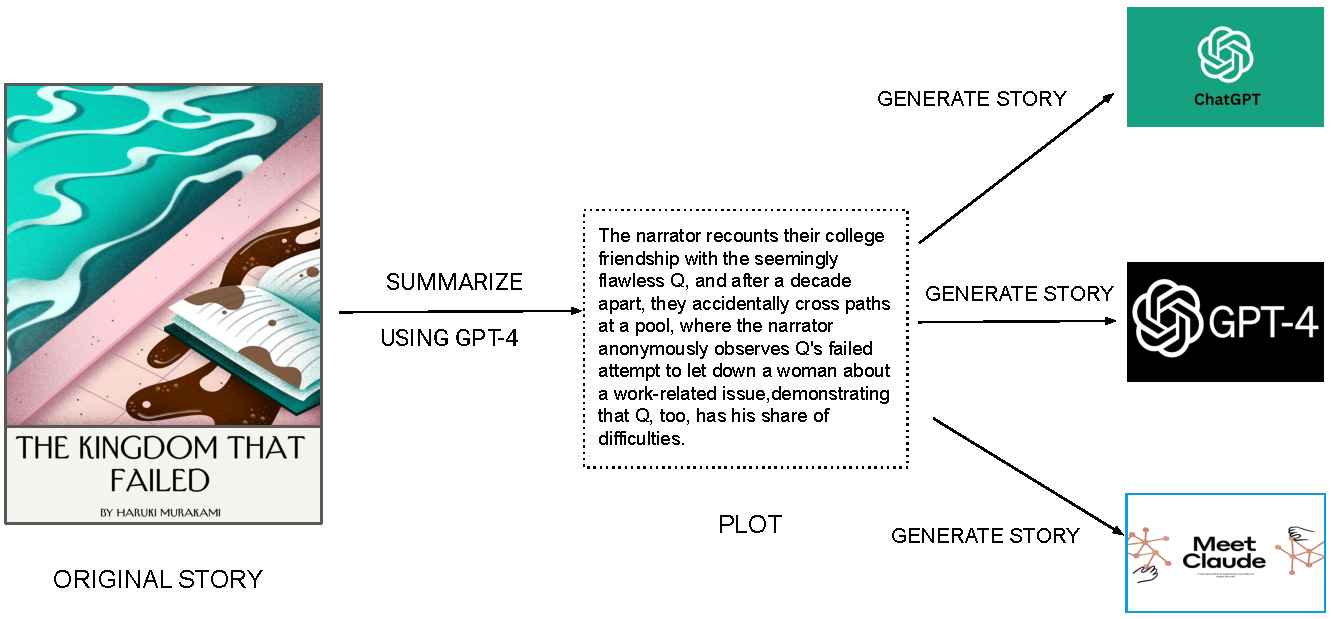
\includegraphics[width=\textwidth]{figures/datapipeline.pdf}
\caption{\label{datapipeline}Pipeline showing how our test set is created for evaluation. For each human-written original NewYorker story, we generate 3 stories from one LLM each, based on the plot of the original story. The plot is a single-sentence summary of the original story automatically generated by GPT-4 and verified by humans.}
\end{figure*}


In order to allow relative evaluation each human-authored narrative is summarized into a single-sentence plot, which is further verified by human evaluators. We then prompt three LLMs: GPT3.5, GPT4, and Claude, to generate a story conditioned on this plot summary. This yields a total of 48 short narratives for absolute evaluation (12 human written; 36 LLM written). Following this, we assign four stories centered around a single plot (one human-authored versus three LLM-authored) to a singular cluster, culminating in a total of 12 clusters. The methodology for creating an individual cluster is illustrated in Figure \ref{datapipeline}. The decision to employ human-authored plot summaries to prompt the LLMs is informed by the recognized shortfall of LLMs in their ability to devise original plotlines, as highlighted in previous research \cite{ippolito2022creative}. Furthermore, the utilization of multiple stories derived from the same plot enables experts to concentrate specifically on the human aspects of creative writing, and enhances their capacity to distinguish human-generated content from AI-produced ones.

In our quest to prevent straightforward parameters from differentiating between stories penned by human authors versus those produced by artificial intelligence (AI), we implemented strategies to ensure comparable story lengths across both classes. Initial experimentation revealed a notable discrepancy: Large Language Models (LLMs), when instructed to generate narratives of a predetermined word count, consistently underperformed, resulting in stories that were invariably more concise than intended. To address this inconsistency, we employed an iterative mechanism, prompting the LLM to iteratively rewrite the initial story until the divergence in word count between the AI-generated and human-composed story was less than 200 for every cluster. Table \ref{promptstory} (Row1) shows the original story prompt, while (Row2) illustrates the subsequent instruction to rewrite the story. We start the iterative process by prompting the LLM to expand the initially generated story. This cycle continued until the narrative length reached the pre-specified threshold or when the iteration count exceeded twenty ($loop\_count > $20). This methodology ensured the creation of AI-written stories with length characteristics more akin to those produced by human authors.

\begin{figure*}
\small
\centering
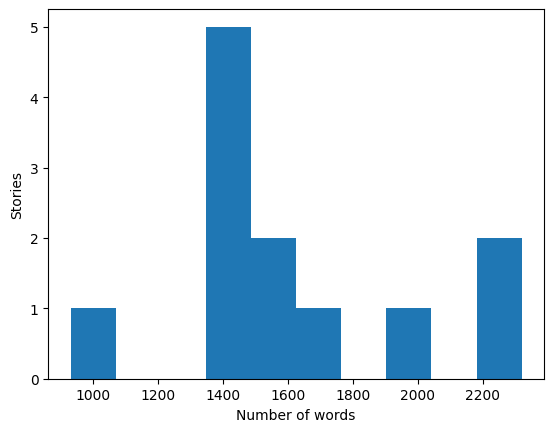
\includegraphics[width=\textwidth]{figures/length.png}
\caption{\label{length} Distribution of word count amongst the stories in our test set}
\end{figure*}


\begin{table}[]
\centering
\small
\def\arraystretch{1.35}
\begin{tabular}{|l|}
\hline
\begin{tabular}[c]{@{}l@{}}Write a New Yorker-style story given the plot below. Make sure it is atleast \textbf{\color{blue}\{\{word\_count\}\}} words. Directly start with the\\ story, do not say things like `Here's the story {[}...{]}:\end{tabular}                                                                                                                                                                                            \\ \hline\hline
\begin{tabular}[c]{@{}l@{}}You wrote the story I gave you below. I requested a story with \textbf{\color{blue}\{\{word\_count\}\}} words, but the story only has\\ \textbf{\color{blue}\{\{current\_word\_count\}\}} words. Can you rewrite the story to make it longer, and closer to the \textbf{\color{blue}\{\{word\_count\}\}} word target\\ I gave you. Directly start with the story, do not say things like `Here's the story {[}...{]}:`\\ \\ Current story: \{\{story\}\}\end{tabular} \\ \hline
\end{tabular}
\vspace{2ex}
\caption{\label{promptstory}Prompt to write the initial story (Row1) vs Prompt to rewrite the initial story to be longer. word\_count represents the number of words in the human written story on a given plot (P) while current\_word\_count represents the number of words in the LLM generated story on the same plot (P)}
\vspace{-7ex}
\end{table}

%     
%     \begin{subfigure}[b]{1.0\textwidth}
%          \centering
%          
\section{\hthree Evaluation}
\label{sec:evaluation}

\begin{table}[t]
    % \captionsetup{font=small}
    \small
    \centering
    % \vspace{-1em}
    \caption{\label{table:gpt} Perplexity (lower is better) of models on the Pile, OpenWebText and
      WikiText-103. GPT-Neo and hybrid \hthree are trained on the Pile, while GPT2 is
      trained on WebText. All models use the same GPT2 tokenizer. We report the
      perplexity of GPT-2 models on the Pile ($^*$) for context, though the performance is not directly comparable since they were trained on different data.}
  %   \vspace{1em}
    {
      \begin{tabular}{@{}|c|c|cc|@{}}
      %   \specialrule{.15em}{.05em}{.05em}
      \hline
        Model & Pile & OpenWebText & WikiText103 \\ % & Training time \\
      %   \specialrule{.15em}{.05em}{.05em}
        \hline
        % GPT-2 small (125M) & 9.8 & 18.2 & -- \\ % & 4.7 days \\
        % H3 (126M) & 18.7 & 4.5 days \\ \hline
        % OPT-125M & -- & -- & -- \\
        GPT-2 small (125M) & 19.0* & 22.6 & 29.9 \\
        GPT-Neo-125M & 9.4 & 22.6 & 26.3 \\
        % GPT3-125M (our replication) & - & - & 24.6 \\
        \textbf{Hybrid H3-125M} & \textbf{8.8} & \textbf{20.9} & \textbf{23.7} \\ \hline %2.7 days \\ \hline
        GPT-2 medium (355M) & 13.9* & 17.0 & 21.8 \\ % & 11.5 days \\
        % H3 (361M) &  &  \\ \hline
        % OPT-350M & -- & -- & -- \\
        % GPT3-355M (our replication) & - & - & 16.6 \\
        \textbf{Hybrid H3-355M} & \textbf{7.1} & \textbf{15.9} & \textbf{16.9} \\ \hline
        GPT-2 XL (1.5B) & 12.4* & 12.9 & 17.0 \\
        % OPT-1.3B & -- & -- & -- \\
        GPT-Neo-1.3B & 6.2 & 13.1 & 13.3 \\
        \textbf{Hybrid H3-1.3B} & \textbf{6.0} & \textbf{12.4} & \textbf{12.5} \\
        \hline
        GPT-Neo-2.7B & 5.7 & 11.7 & 11.5 \\
        \textbf{Hybrid H3-2.7B} & \textbf{5.4} & \textbf{11.0} & \textbf{10.6} \\
        \hline
      \end{tabular}
    }
    % \vspace{-1.5em}
  \end{table}

\begin{table}[t]
    % \captionsetup{font=small}
    \scriptsize
    \centering
    % \vspace{-1em}
    \caption{\label{table:superglue_zeroshot_logit} Zero-shot acc.\ on SuperGLUE with logit scoring. Best results in bold, second best underline. }
    %   \vspace{1em}
    {
        \begin{tabular}{@{}|c|cccccccc|c|@{}}
            \hline
        %   \specialrule{.15em}{.05em}{.05em}
        Model & WSC & WIC & RTE & CB & MultiRC & ReCoRD & BoolQ & COPA & Average \\ % & Training time \\
        %   \specialrule{.15em}{.05em}{.05em}
        \hline
        % GPT-2 small (125M) & -- & -- & -- & -- & -- & -- & -- & -- & -- \\ % & 4.7 days \\
        % H3 (126M) & 18.7 & 4.5 days \\ \hline
        OPT-125M & \textbf{39.4} & \underline{52.0} & 48.7 & 37.4 & \underline{58.9} & \underline{44.9} & \underline{59.6} & \underline{60.0} & 50.1 \\
        GPT-Neo-125M & \underline{36.5} & \textbf{53.6} & \underline{53.1} & \underline{41.1} & \textbf{59.9} & 39.6 & \textbf{62.2} & \underline{60.0} & \underline{50.8} \\
        % \textbf{\hthree-125M} & 0.0 & 0.0 & 47.3 & 8.9 & 0.0 & -- & 37.8 & 51.0 & 20.7 \\ %2.7 days \\ \hline
        \textbf{Hybrid \hthree-125M} & \textbf{39.4} & 51.4 & \textbf{59.2} & \textbf{48.2} & 51.4 & \textbf{55.0} & \underline{59.6} & \textbf{67.0} & \textbf{53.9} \\ \hline %2.7 days \\ \hline
        GPT-2 medium (355M) & \underline{50.0} & \textbf{52.0} & 51.3 & 28.6 & \textbf{59.5} & \underline{53.3} & \underline{61.0} & \underline{65.0} & 52.6 \\
        % H3 (361M) &  &  \\ \hline
        OPT-350M & \textbf{53.5} & 50.8 & \underline{53.4} & \underline{35.7} & \underline{58.9} & 51.4 & 60.9 & 60.0 & \underline{53.1} \\
        \textbf{Hybrid \hthree-355M} & 37.5 & \underline{51.7} & \textbf{55.2} & \textbf{41.1} & \textbf{59.5} & \textbf{62.3} & \textbf{61.5} & \textbf{69.0} & \textbf{54.7} \\ \hline
        % GPT-2 (1.5B) & 14.4 & \textbf{36.5} & \underline{49.1} & \underline{8.9} & 0.5 & \underline{44.0} & \underline{46.6} & 59.0 & 32.4 \\
        OPT-1.3B & 36.5 & 49.5 & \textbf{53.4} & \textbf{39.3} & \textbf{58.3} & \underline{61.8} & 55.0 & \underline{69.0} & \underline{52.9} \\
        GPT-Neo-1.3B & \underline{41.3} & \underline{50.0} & \underline{52.3} & \underline{33.9} & 57.9 & 55.5 & \underline{59.9} & 66.0 & 52.1 \\
        \textbf{Hybrid \hthree-1.3B} & \textbf{52.9} & \textbf{50.3} & \textbf{53.4} & \underline{33.9} & \underline{58.2} & \textbf{67.8} & \textbf{61.7} & \textbf{74.0} & \textbf{56.5} \\ \hline
        OPT-2.7B & \textbf{51.0} & \underline{50.8} & 50.5 & \underline{41.1} & 57.4 & \underline{65.9} & 60.9 & 66.0 & \underline{55.5} \\
        GPT-Neo-2.7B & \underline{37.5} & 50.0 & \underline{52.3} & \textbf{50.0} & \textbf{59.1} & 60.0 & \textbf{61.1} & \underline{67.0} & 54.6 \\
        \textbf{Hybrid \hthree-2.7B} & 36.5 & \textbf{51.3} & \textbf{57.0} & 37.5 & \underline{58.7} & \textbf{71.3} & \textbf{61.1} & \textbf{81.0} & \textbf{56.8} \\ \hline
        \end{tabular}
    }
    % \vspace{-1.5em}
\end{table}
\begin{table}[t]
    % \captionsetup{font=small}
    \scriptsize
    \centering
    % \vspace{-1em}
    \caption{\label{table:superglue_fewshot_logit} 3-shot acc.\ on SuperGLUE with logit scoring. Best results in bold, second best underline. }
    %   \vspace{1em}
    {
        \begin{tabular}{@{}|c|cccccccc|c|@{}}
            \hline
        %   \specialrule{.15em}{.05em}{.05em}
        Model & WSC & WIC & RTE & CB & MultiRC & ReCoRD & BoolQ & COPA & Average \\ % & Training time \\
        %   \specialrule{.15em}{.05em}{.05em}
        \hline
        % GPT-2 small (125M) & -- & -- & -- & -- & -- & -- & -- & -- & -- \\ % & 4.7 days \\
        % H3 (126M) & 18.7 & 4.5 days \\ \hline
        OPT-125M & 36.5 & \textbf{50.2} & 47.3 & \underline{44.6} & \textbf{57.9} & \underline{44.9} & 41.9 & 60.0 & \underline{47.9} \\
        GPT-Neo-125M & \underline{38.5} & \underline{50.0} & \underline{53.1} & 17.9 & \underline{56.3} & 39.6 & \textbf{62.1} & \underline{60.0} & 47.2 \\
        \textbf{Hybrid \hthree-125M} & \textbf{43.3} & 49.1 & \textbf{58.1} & \textbf{51.8} & 48.9 & \textbf{55.0} & \underline{56.1} & \textbf{67.0} & \textbf{53.7} \\ \hline %2.7 days \\ \hline
        GPT-2 medium (355M) & 36.5 & \textbf{50.5} & \underline{48.0} & 8.9 & 43.5 & \underline{53.3} & 58.8 & \underline{65.0} & 45.6 \\
        % H3 (361M) &  &  \\ \hline
        OPT-350M & \underline{37.5} & \underline{50.0} & 45.8 & \textbf{44.6} & \underline{49.8} & 51.4 & \textbf{61.7} & 60.0 & \underline{50.1} \\
        \textbf{Hybrid \hthree-355M} & \textbf{42.3} & 47.5 & \textbf{50.5} & \underline{28.6} & \textbf{59.7} & \textbf{62.3} & \underline{60.5} & \textbf{69.0} & \textbf{52.6} \\ \hline
        % GPT-2 (1.5B) & \underline{36.5} & 36.5 & \textbf{56.7} & 41.1 & 6.1 & 43.8 & \underline{53.7} & 61.0 & 41.9 \\
        OPT-1.3B & \textbf{44.2} & \textbf{51.1} & \underline{53.4} & 16.1 & \textbf{59.9} & \underline{62.1} & 38.3 & \underline{70.0} & 49.4 \\
        GPT-Neo-1.3B & 35.6 & \underline{50.6} & 47.3 & \textbf{32.1} & \textbf{59.9} & 55.7 & \textbf{61.2} & 67.0 & \underline{51.2} \\
        \textbf{Hybrid \hthree-1.3B} & \underline{36.5} & 49.2 & \textbf{55.2} & \underline{23.2} & \underline{59.3} & \textbf{67.6} & \underline{56.9} & \textbf{76.0} & \textbf{53.0} \\ \hline
        OPT-2.7B & \underline{44.2} & \underline{50.5} & \textbf{53.4} & 17.9 & \underline{59.2} & \underline{66.0} & \textbf{62.0} & \underline{71.0} & \underline{53.0} \\
        GPT-Neo-2.7B & \textbf{49.0} & \textbf{51.9} & \underline{51.6} & \underline{21.4} & 57.0 & 60.0 & 56.0 & 68.0 & 51.9 \\
        \textbf{Hybrid \hthree-2.7B} & 36.5 & 45.6 & 47.3 & \textbf{46.4} & \textbf{59.4} & \textbf{71.1} & \underline{60.6} & \textbf{77.0} & \textbf{55.5} \\ \hline
        \end{tabular}
    }
    % \vspace{-1.5em}
\end{table}

To understand how well capturing the synthetics in Section~\ref{sec:synthetics} translates to language modeling, we train two hybrid hybrid \hthree-attention language models at sizes 125M, 355M, 1.3B, and 2.7B, and we evaluate their performance against Transformers.
The hybrid models match or exceed the quality of Transformers in perplexity and zero/few-shot learning.
We also validate that \hthree models retain strong performance on non-text sequence modeling.
Appendix~\ref{sec:app_additional_experiments} contains additional experiments on more datasets, length extrapolation, and scaling with data.

\subsection{Language Modeling}
\label{subsec:language_modeling}

We compare hybrid \hthree-attention language models against Transformer-based language models.
We evaluate language modeling performance using perplexity, zero-shot learning, and few-shot learning performance.
Hybrid \hthree models outperform Transformers, which suggests that closing the gap between SSMs and attention on the synthetic languages translates to real language modeling capabilities.
We also report the generation speed of hybrid \hthree models compared to Transformers; since SSMs are recurrent models, they can generate tokens \num{2.4$\times$} faster than Transformers.
Appendix~\ref{sec:app_additional_experiments} shows performance of pure \hthree language models on these same evaluation metrics.

\paragraph{Setup}
We train hybrid models at sizes 125M, 355M, 1.3B, and 2.7B on the Pile~\citep{gao2020pile} for 400B tokens.
We compare against checkpoints of equivalent sizes from
Open-AI~\citep{radford2019language} and GPT-Neo\footnote{There
  is no pretrained GPT-Neo at the 350M size.}~\citep{gpt-neo},
from HuggingFace~\citep{wolf-etal-2020-transformers}.


\paragraph{Perplexity}
Table \ref{table:gpt} shows perplexity on the Pile~\citep{gao2020pile}, OpenWebText~\citep{Gokaslan2019OpenWeb}, and WikiText-103~\citep{merity2016pointer}. 
On the Pile, our 125M hybrid model outperforms GPT-Neo, which was also trained on the Pile.
Our hybrid models also outperform GPT-Neo models and GPT-2 models on zero-shot transfer to OpenWebText and WikiText103.
We report the PPL of GPT-2 models for context, though the performance is not directly comparable since they were trained on different data.

\paragraph{Zero- and Few-shot Performance}
We compare the zero- and few-shot performance of hybrid \hthree language models against OPT~\citep{zhang2022opt}, GPT-Neo, and GPT-2 models, where public checkpoints are available.
We report performance with rank classification on the logits of the possible choices (see Appendix~\ref{sec:app_generation} for raw generation).
Table~\ref{table:superglue_zeroshot_logit} reports zero-shot performance on the SuperGLUE benchmark, and Table~\ref{table:superglue_fewshot_logit} reports the 3-shot performance.
Following the perplexity results, the hybrid language models outperform or match the best the Transformer baseline on more than half the tasks.

\begin{table}[t]
\centering
% \begin{table}[h]
    % \captionsetup{font=small}
    \small
    \centering
    % \vspace{-1em}
    \caption{\label{table:training_time} Inference throughput on A100 80GB, 1.3B models.
    Batch size 64, prompt length 512, 1024, or 1536, and generating 128 tokens
    per sequence in the batch (i.e., 64 $\times$ 128 tokens in a batch). Hybrid
    \hthree is up to 2.4$\times$ faster than a Transformer of similar size in inference. The
    difference is larger for longer sequences.}
    %   \vspace{1em}
    {
        \begin{tabular}{@{}|c|c|c|c|@{}}
            \hline
        %   \specialrule{.15em}{.05em}{.05em}
        Tokens/s & Prompt length 512 & Prompt length 1024 & Prompt length 1536 \\ % & Training time \\
        %   \specialrule{.15em}{.05em}{.05em}
        \hline
        Transformer-1.3B & 1340 & 770 & 520 \\
        % GPT-2 Small (FlashAttention~\citep{dao2022flashattention}) & -- & -- \\ 
        % GPT-2 Small (FasterTransformer~\citep{}) & N/A & -- \\ \hline
        Hybrid \hthree-1.3B & 1980 & 1580 & 1240 \\ \hline
        \end{tabular}
    }
    % \vspace{-1.5em}
% \end{table}
\end{table}
\paragraph{Language Modeling Inference}
Finally, since SSMs are recurrent models, they admit faster text generation than Transformers.
Table~\ref{table:training_time} shows inference throughput of a 1.3B-parameter hybrid model compared to a Transformer.
The hybrid model has up to \num{2.4$\times$} higher throughput.



%%% Local Variables:
%%% mode: latex
%%% TeX-master: "../main"
%%% End:

\section{Converting expert questions to quantifiable Natural language instructions} \label{sec:prompting}

\begin{table*}[!h]
\centering
\small
\def\arraystretch{1.15}
\begin{tabular}{|l|l|}
\hline
\begin{tabular}[c]{@{}l@{}}Expert \\ Measure\end{tabular}               & Does the writer make the fictional world believable at the sensory level?                                                                                                                                     \\ \hline
\begin{tabular}[c]{@{}l@{}}Expanded\\ Expert\\ Measure (M)\end{tabular} & \begin{tabular}[c]{@{}l@{}}Sensory details pertain to the five senses - sight, sound, touch, taste, and smell. An effective \\ writer can use these elements to paint a detailed picture of the story's environment, making\\ it feel tangible and real to the reader.\\ \\ For example, describing the specific colors and shapes in a scene, the sounds that fill a space,the \\ textures and temperatures that a character comes into contact with, the flavors of the food they \\ eat, or the scents that fill the air, can all contribute to creating a sensory-rich and believable world.\\ \\ By stimulating the reader's senses, the writer can make the reader feel as though they're \\ experiencing the events of the story firsthand.This level of detail contributes to the believability of\\ the world, even if it's a completely fictional or fantastical setting. It helps the reader to suspend\\ disbelief and become more deeply invested in the narrative.\end{tabular} \\ \hline
\begin{tabular}[c]{@{}l@{}}Human\\ Instruction\end{tabular}             & \begin{tabular}[c]{@{}l@{}}\{\{M\}\}\\ \\ Based on the story that you just read, answer the following question.\\ \textit{\color{blue}Does the writer make the fictional world believable at the sensory level?}\end{tabular}                                                                       \\ \hline
\begin{tabular}[c]{@{}l@{}}LLM\\ Instruction\end{tabular}               & \begin{tabular}[c]{@{}l@{}}\{\{M\}\}\\ \\ Given the story above, list out the elements in the story that call to each of the\\ five senses. Then overall, give your reasoning about the question below and give\\ an answer to it between 'Yes' or 'No' only\\ \\ \textit{\color{blue} Q) Does the writer make the fictional world believable at the sensory level?}\end{tabular}                                                                                                                                                                                                                                 \\ \hline
\end{tabular}
\vspace{2ex}
\caption{\label{prompting}Expert suggested question for World Building and setting (Row1) ; Elucidated prompt designed for other expert humans (Row2); Elucidated quantifiable prompt designed for Large Language Models that elicit Chain of Thought Reasoning(Row3) }
\vspace{-5ex}
\end{table*}

An expert suggested questions for empirically evaluating creative writing might frequently elicit ambiguity in Large Language Models or even other creative writing experts. In order for LLMs or other experts to comprehend the suggested questions in Table \ref{CreativityTest} we attempt at expanding them by adding more details. Recent pre-trained LLMs (e.g., GPT-4 \cite{OpenAI2023GPT4TR} GPT3.5 \cite{ChatGPT}) can engage in fluent, multi-turn conversations out of the box, substantially lowering the data and programming-skill barriers to creating passable conversational user experiences. People can improve LLM outputs by prepending prompts—textual instructions and examples of their desired interactions—to LLM inputs. The prompts steer the model towards generating the desired outputs, raising the ceiling of what conversational UX is achievable for non-AI experts.To elucidate these questions we prompt GPT4 with the following instruction \textit{What do creative experts mean when they say the following: \{\{expert question\}\}}. Once GPT4 gives a response 3 domain experts carefully verify the response and edit it where required in order to convert it into a detailed natural language instruction. Table \ref{prompting} (Row2) shows the human-verified GPT4 elucidated instruction in response to the input prompt.

Prior work \cite{wei2022chain} has shown how generating a \textit{chain of thought} -- a series of intermediate reasoning steps -- significantly improves the ability of large language models to perform complex reasoning. Taking advantage of this we design the prompts for large language models in a slightly different fashion as that of expert humans as can be seen in Table \ref{prompting}. To help the model make an informed decision we first ask it to list out elements specific to any given test such as ``elements in the story that call to each of the five senses" for the World Building and setting test followed by asking it decide overall and then provide its reasoning before choosing an answer between `Yes' or `No'.More examples of Human and LLM instructions for the remaining 13 tests are provided in Appendix \ref{appendix}
\begin{table*}
\small
\centering
\def\arraystretch{1.35}
\begin{tabular}{|l|l|l|l|l|l|}
\hline
      Dimension      & Test & GPT3.5 & GPT4 & Claudev1.3 & Human                         \\ \hline
\multirow{5}{*}{Fluency} & Understandability \& Coherence                                                     &  15.0      & 30.0     &      55.0     &  \textbf{90.0}     \\ \cline{2-6}
 & Narrative Pacing                                                                   &  10.0      &   50.0   &       70.0    &   \textbf{90.0}   \\ \cline{2-6}
 & Scene vs Exposition                                                                &  10.0      &   60.0   &     65.0      &  \textbf{85.0}     \\ \cline{2-6}
 & \begin{tabular}[c]{@{}l@{}}Literary Devices \& Language Proficiency\end{tabular} &   5.0     &   40.0   &     15.0      & \textbf{80.0}      \\ \cline{2-6}
 & Narrative Ending                                                                   & 10.0       & 20.0     &      45.0     &  \textbf{85.0}     \\ \hline\hline
\multirow{3}{*}{Flexibility} & Emotional Flexibility                                                              &   20.0     &  25.0    &    55.0       &  \textbf{90.0}    \\ \cline{2-6}
& Perspective \& Voice Flexibility                                                   &  10.0     &   20.0   &     25.0      &  \textbf{70.0}     \\ \cline{2-6}
& Structural Flexibility                                                             &  15.0      &  30.0    &    35.0       & \textbf{90.0}     \\ \hline\hline
\multirow{3}{*}{Originality} & Originality in Form \& Structure                                                   & 0.0       &   15.0   &     0.0      &  \textbf{60.0}     \\ \cline{2-6}
& Originality in Thought                                                             &   5.0     &   60.0   &     35.0      &  \textbf{90.0}     \\ \cline{2-6}
& Originality in Theme \& Content                                                    &  0.0      &  30.0    &     10.0      &  \textbf{85.0}     \\ \hline\hline
\multirow{3}{*}{Elaboration} &  World Building \& Setting                                                          &   15.0     &   35.0   &    65.0       &  \textbf{90.0}    \\ \cline{2-6}
& Character Development                                                              &   10.0     &  20.0   &  25.0        &  \textbf{75.0}    \\ \cline{2-6}
& Rhetorical Complexity                                                              &    5.0    &  10.0    &    10.0       &  \textbf{90.0}    \\ \hline
\end{tabular}
\vspace{2ex}
\caption{\label{absolutehumaneval}\textbf{Absolute Evaluation}: Average passing rate on individual creativity test obtained from 8 creative writing experts across all stories in our test set authored by GPT3.5,GPT4,Claude and Humans}

\begin{tabular}{|l|l|l|l|l|}
\hline
                                                                               & GPT3.5 & GPT4 & Claudev1.3 & Human \\ \hline
\begin{tabular}[c]{@{}l@{}}Relative Ranking Based on Preference\end{tabular} & 3.45   & 3.0  & 2.35       & 1.2   \\ \hline
\end{tabular}
\vspace{2ex}
\caption{\label{relativehumaneval} \textbf{Relative Evaluation}:Average ranking provided by 8 creative writing experts based on their subjective preference across all stories in our test set authored by GPT3.5,GPT4,Claude and Humans}
\end{table*}
% \begin{figure*}
%     \centering
%     \begin{subfigure}[b]{1.0\textwidth}
%          \centering
%          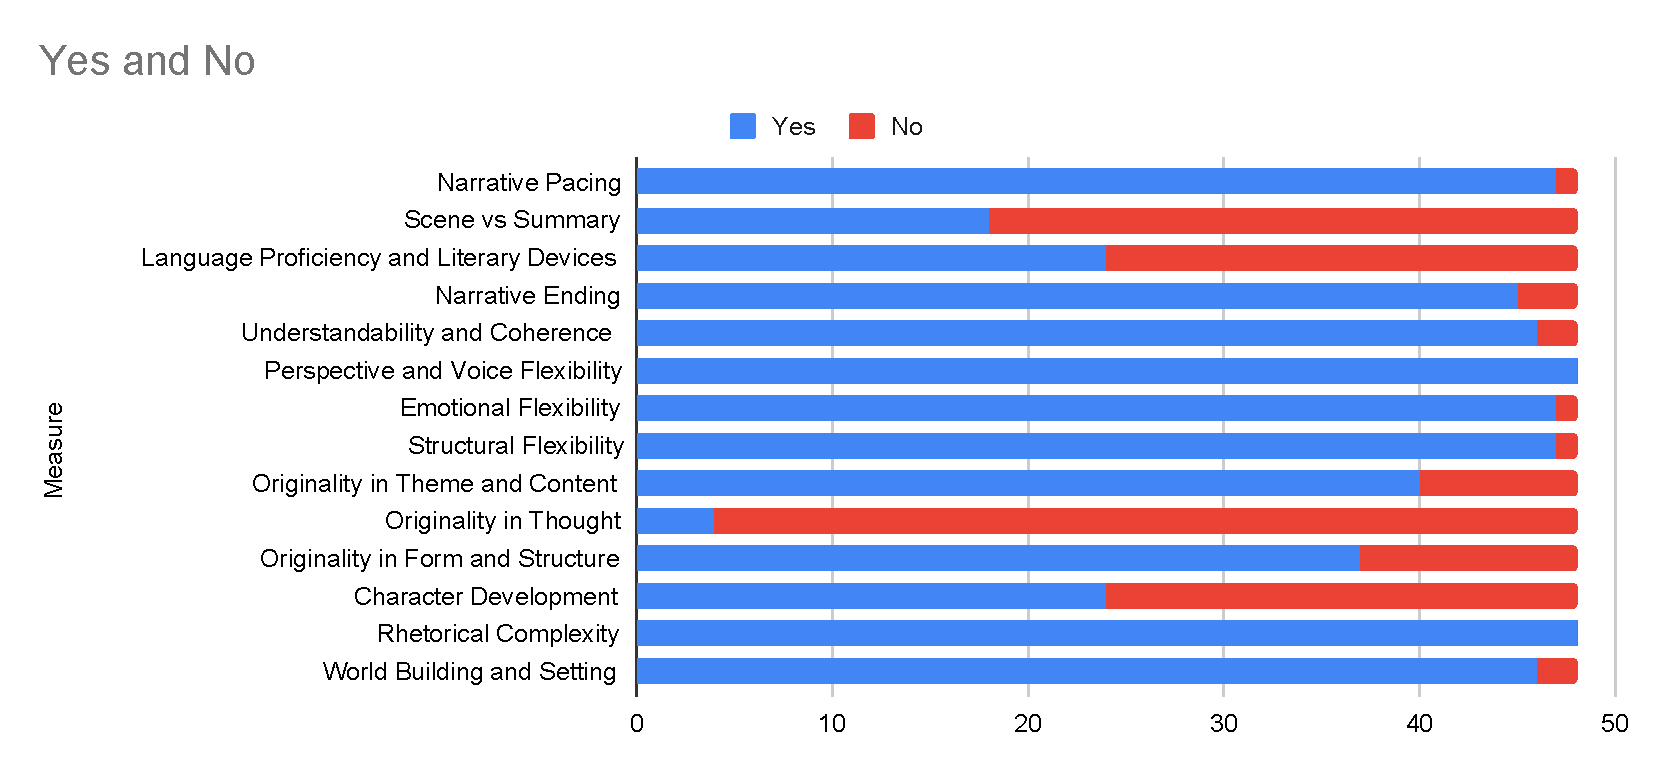
\includegraphics[width=\textwidth]{figures/GPT3.5.pdf}
%          \caption{Binary judgements across 48 stories from GPT3.5 on 14 tests}
%          \label{fig:GPT3.5YesNo}
%     \end{subfigure}
%     % \hfill
%     \begin{subfigure}[b]{1.0\textwidth}
%         \centering
%         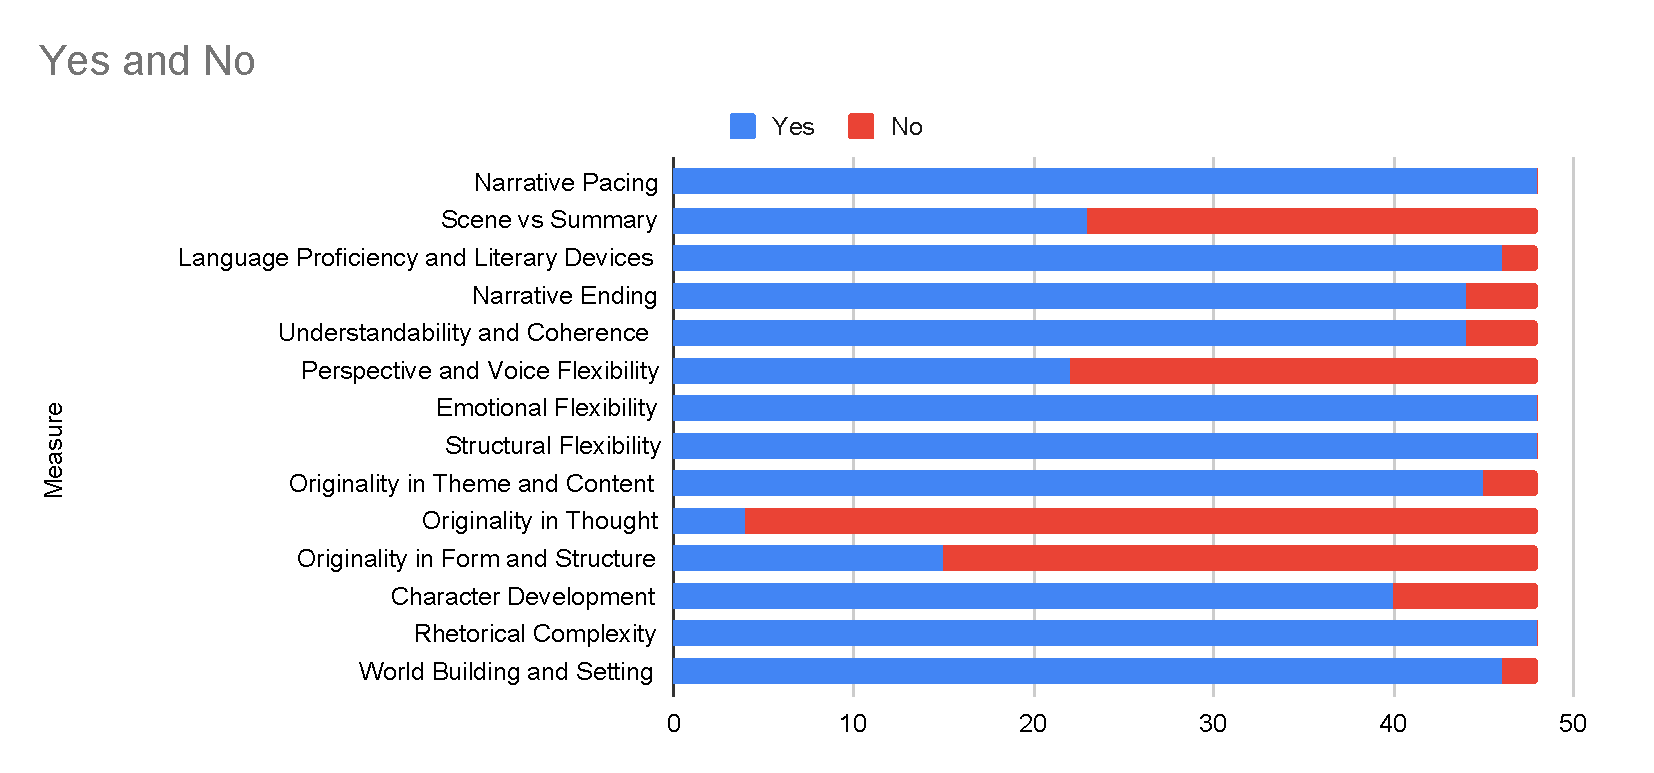
\includegraphics[width=\textwidth]{figures/GPT4.pdf}
%         \caption{Binary judgements across 48 stories from GPT4 on 14 tests}
%         \label{fig:categories}
%     \end{subfigure}
%     \label{fig:GPT4YesNo}
%       \begin{subfigure}[b]{1.0\textwidth}
%         \centering
%         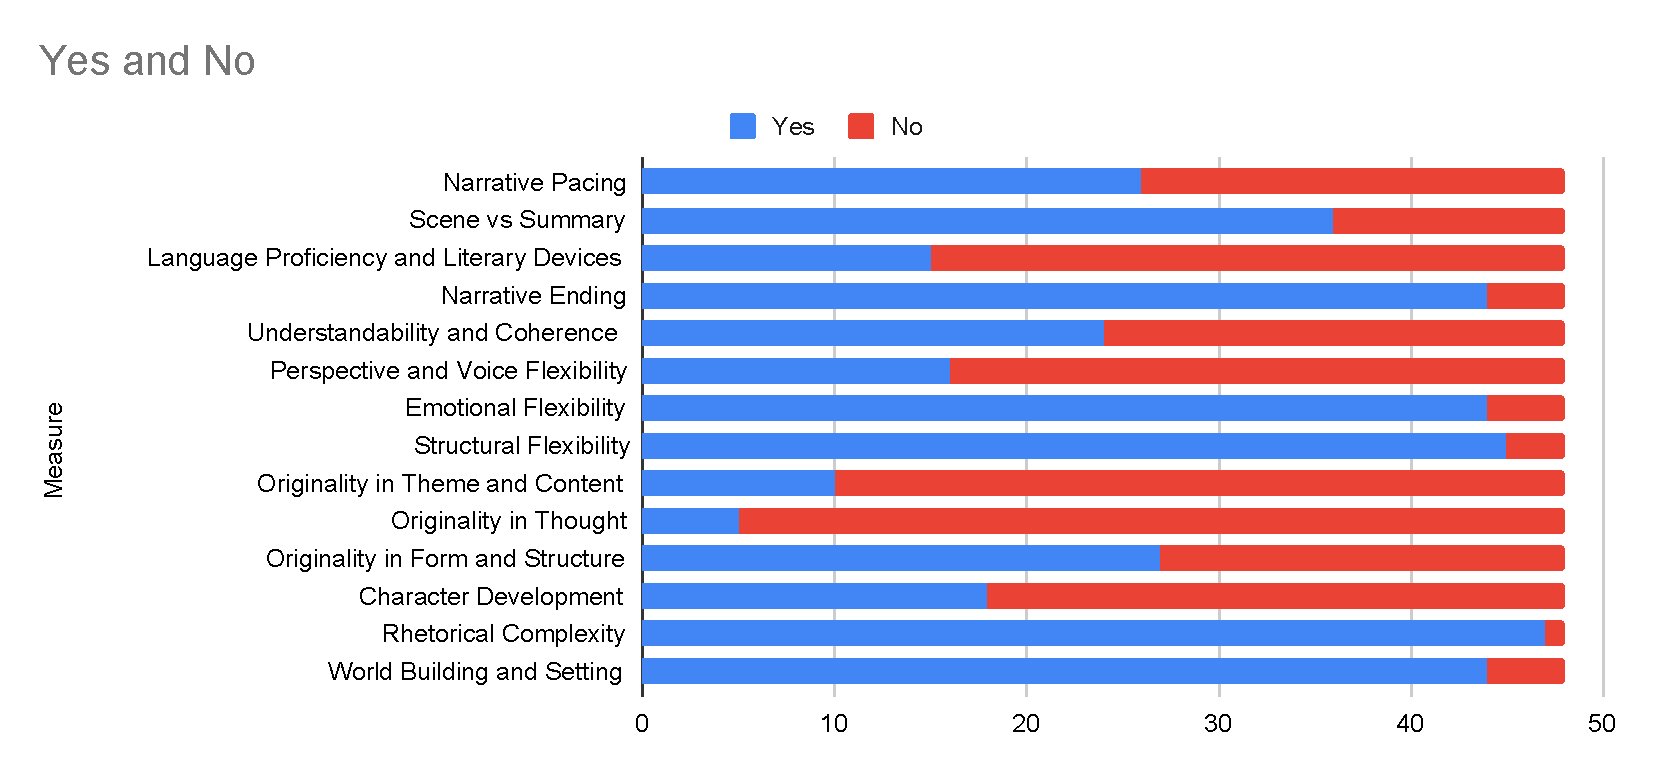
\includegraphics[width=\textwidth]{figures/Claude.pdf}
%         \caption{Binary judgements across 48 stories from Claude on 14 tests}
%         \label{fig:categories}
%     \end{subfigure}
%     \label{fig:ClaudeYesNo}
% \end{figure*}


\section{Conclusion}
\section{Acknowledgments}
\section{Appendices}\label{appendix}



\bibliographystyle{ACM-Reference-Format}
\bibliography{sample-base}
\end{document}
\endinput
%%
%% End of file `sample-authordraft.tex'.
